\documentclass[11pt]{article}
\usepackage[margin=1.1in]{geometry}
\usepackage{amsmath,amssymb,amsthm}
\usepackage{graphicx}
\usepackage{booktabs}
\usepackage[round]{natbib}
\usepackage{hyperref}
\hypersetup{hidelinks}
\usepackage{microtype}

\newtheorem{theorem}{Theorem}
\newtheorem{proposition}[theorem]{Proposition}
\newtheorem{corollary}[theorem]{Corollary}
\newtheorem{lemma}[theorem]{Lemma}
\theoremstyle{remark}
\newtheorem{remark}[theorem]{Remark}

\newcommand{\E}{\mathbb{E}}
\newcommand{\Prob}{\mathbb{P}}
\newcommand{\KL}{\mathrm{KL}}
\newcommand{\I}{\mathrm{I}}
\newcommand{\given}{\,|\,}
\newcommand{\F}{\mathcal{F}}
\newcommand{\Dn}{D_n}
\newcommand{\Reg}{\mathcal{R}}
\newcommand{\Loss}{\mathcal{L}}

\newif\ifanon
\ifdefined\anonymous\anontrue\fi

\title{An Empirical Study of the Conformal Information Gap}
\ifanon
\author{Anonymized for double-blind review}
\else
\author{Peter Cotton\\\texttt{peter.cotton@microprediction.com}}
\fi
\date{August 2026}

\begin{document}
\maketitle

\begin{abstract}
Every forecasting architecture restricts the information available to its predictive law.
Under logarithmic loss the irreducible cost of replacing the full input by a retained
representation is exactly the conditional mutual information between outcome and input given
the representation. Following a companion note, we call it the information gap. For a single pooled residual law the gap
is the mutual information between residual and input, and pooling after any invertible
state-dependent change of coordinates has the analogous gap in the transformed coordinates.
Conformal calibration can improve estimation and provide a coverage certificate, but it
cannot recover predictive information excluded by the retained representation. We apply the decomposition to a
nested grammar of online transformations on 572 economic series. Conditional scale is the
largest and most reliable component of the measured architecture gain, and, holding the point
predictor fixed, scale-normalized empirical pooling beats raw pooling on 90 percent of the
series under a quantile approximation to CRPS. The value of residual pooling depends jointly
on the coordinates, the residual-law estimator, and the scoring rule.
\end{abstract}

\section{Introduction}\label{sec:intro}

This paper asks when residual pooling is an effective component of probabilistic
forecasting. The motivating application is an online distributional time-series forecaster
built from chained transformations, but the underlying question is general: what predictive
value is lost when a forecast uses only a representation $T(X)$ of the available information
$X$? Under logarithmic loss that loss has an exact decomposition, and we call its irreducible
representation component the \emph{information gap}. \ifanon A recent note, blinded for
review, introduces the gap for a single pooled residual law. \else A companion note
introduces the gap for a single pooled residual law \citep{cotton2026marginally}. \fi This
paper extends the definition to arbitrary retained representations and keeps the treatment
self-contained for convenience.

A forecasting method is partly a model and partly a decision about what information the forecast
is allowed to use. A global residual distribution remembers no input-dependent residual state. A
volatility model remembers an estimated scale. A tree ensemble remembers a partition and its
fitted leaf values. A state-space filter remembers a posterior state. A neural forecaster
remembers a learned embedding. In each case the predictive law is measurable with respect to a
representation $T(X)$ of the available information $X$.

We ask a simple question:
\begin{quote}
What is the predictive cost of replacing the full information $X$ by a representation $T(X)$?
\end{quote}

Under logarithmic score the answer is exact. Let $Z$ be the target, let $p(z\given x)$ denote the
true conditional density, and let $q(z\given T)$ be any predictive density that can depend on $X$
only through $T$. Then
\begin{equation}\label{eq:decomp}
\E\log\frac{p(Z\given X)}{q(Z\given T)}
=\underbrace{\I(Z;X\given T)}_{\text{representation regret}}
+\underbrace{\E_T\KL\big(P_{Z|T}\,\|\,Q_{Z|T}\big)}_{\text{within-representation regret}} .
\end{equation}
Here $\I(Z;X\given T)$ is the conditional mutual information between $Z$ and $X$ given $T$,
$P_{Z|T}$ is the true conditional law of $Z$ given $T$, and $Q_{Z|T}$ is the forecast. Formal definitions are collected in
Section~\ref{sec:decomposition}. The first term is the Bayes
value of the information in $X$ that is absent from $T$. We call it the \emph{information
gap}, or floor, of the representation. It vanishes precisely when $T$ is
sufficient for predicting $Z$. The second term measures how far the fitted
forecast lies above the best forecast permitted by the architecture. Global residual pooling deliberately uses a coarse residual representation. The question is
whether its reduced estimation burden compensates for the resulting representation floor.

Identity \eqref{eq:decomp} is classical in substance. It is a conditional relative-entropy
decomposition, closely related to value-of-information results, Blackwell sufficiency, and
proper-scoring-rule entropy
\citep{lindley1956measure,degroot1962uncertainty,blackwell1953equivalent,grunwald2004game}. It
is also the misspecified-model decomposition of \citet{white1982maximum}. The model class is
the family of all predictive laws measurable with respect to $T$, and its pseudo-true member
is $p(\cdot\given T)$. For such an information-restricted class the irreducible
misspecification error takes the closed form $\I(Z;X\given T)$.

To our knowledge this decomposition has not been stated for conformal prediction. It applies
there with unusual ease, because residual pooling fixes $T$ by construction. The irreducible
term becomes the mutual information $\I(R;X)$ between residual and input. We state the decomposition for pooled residual systems and, in
Theorem~\ref{thm:transformpool}, for pooling in any state-dependent coordinates. We then
price fitted architecture increments against the decomposition on a large benchmark, and we
separate the part of a residual method's predictive shortfall due to its coordinates from the
part due to its estimator. The accounting applies to any forecasting architecture. Conformal
prediction is the running case study because its representation choice is explicit.

We now specialize. Let the target be a real-valued outcome $Y$, fix a point predictor
$\hat\mu(x)$, and define the residual
\[
R=Y-\hat\mu(X).
\]
A single-shape residual forecast uses one law $H$ for $R$ at every input and reports
\[
q_H(y\given x)=h\big(y-\hat\mu(x)\big).
\]
The point forecast may be highly adaptive, but the residual-shape representation is trivial.
Conditional on the fixed location model, the best input-blind residual law is the marginal law
$P_R$, and its log-score regret relative to the conditional residual oracle is
\[
\I(R;X).
\]

Signed-residual conformal predictive systems (CPS) converge to this marginal residual law under
standard conditions \citep{vovk2019nonparametric}. Thus they are population-optimal within
the input-blind residual class. The representation floor remains. Ordinary absolute-residual
intervals impose an additional symmetrization restriction.

The distinction between representation and calibration is central. A conformal procedure can
change a fitted CDF, quantiles, intervals, and therefore proper scores. It may improve or worsen
the estimation term. What it cannot do is reduce $\I(R;X\given T)$ while leaving $T$ unchanged. A
conformal method reduces this floor only when its score, normalization, partition, localization
rule, or learned embedding actually enlarges the retained representation.

The same decomposition gives a precise architecture-selection criterion. If $T_A$ is a coarsening
of $T_B$, the oracle advantage of $T_B$ is the additional predictive information
$\I(Z;T_B\given T_A)$. At finite samples this gain competes with the richer method's extra
within-representation excess risk. Under a prior on Nature, the richer method wins exactly when its information
advantage exceeds its statistical cost. This yields a concrete theoretical explanation for why
boosted conditional-distribution learners can outperform global residual pooling under priors
concentrated on learnable heteroscedastic or interaction structure
\citep{friedman2001greedy,chen2016xgboost,duan2020ngboost}.

Our claims divide accordingly. The value-of-information lemma, its proper-score
analogue, monotonicity under refinement, and the approximation--estimation split are classical
or immediate. We state them with explicit regularity conditions and with learned
representations
treated conditionally on training data. Our own contributions are the transform-pooling
theorem, which prices every pooled-residual scheme by the coordinates in which it pools, and
two experiments built on it: a nested-ladder ablation over 572 economic series
(Figure~\ref{fig:ladder}) and a matched-predictor comparison that separates the cost of a
method's coordinates from the cost of its estimator.

\section{Related ideas}\label{sec:related}

\subsection{Value of information, sufficiency, misspecification, and proper scores}

Under log loss, the reduction in Bayes risk obtained by observing additional information is a
mutual information. This is classical \citep{lindley1956measure,degroot1962uncertainty}.
Blackwell's comparison of experiments formalizes when one information structure is more useful
than another for every decision problem \citep{blackwell1953equivalent}. For logarithmic
prediction, the value of a refinement has the explicit form of conditional mutual
information.

The same identity has ancestors in at least three further literatures. In misspecified-model
theory, maximum likelihood converges to the KL projection of the truth onto the model class
\citep{white1982maximum}. Here the class is the set of $T$-measurable predictive laws. The
pseudo-true member is $P_{Z|T}$, and the projection distance is $\I(Z;X\given T)$. In
sufficient dimension reduction, one seeks $T(X)$ with $Z\perp X\given T(X)$
\citep{li1991sliced,fukumizu2004dimensionality}. That is exactly the zero-floor condition
$\I(Z;X\given T)=0$. The decomposition supplies the graded log-score price of
insufficiency, in the spirit of information-theoretic reductions that minimize lost mutual
information \citep{globerson2003sufficient}. In the information bottleneck
\citep{tishby1999information}, the Markov chain $Z-X-T$ gives
$\I(Z;X)=\I(Z;T)+\I(Z;X\given T)$, so minimizing the floor is maximizing retained
predictive information. The bottleneck penalizes representation complexity by $\I(X;T)$. We
penalize finite-sample estimation and certification cost instead, and the two need not
coincide.

Akaike's programme of choosing the fitted model with smallest estimated expected KL
discrepancy \citep{akaike1974new} likewise separates approximation error from estimation
optimism. Our refinement is that for information-restricted classes the approximation term is
identified exactly.

We apply these facts to the design of forecasters. Here $T$ is the state a forecasting
method retains, not a statistic an analyst chooses afterward. The decomposition then
separates two errors: the error built into that choice of state, and the error of fitting
within it.

\subsection{Calibration and sharpness}

The forecasting literature distinguishes calibration from sharpness and advocates maximizing
sharpness subject to calibration \citep{gneiting2007probabilistic,dawid1984present}. Proper
scores combine these considerations into a single decision criterion
\citep{gneiting2007strictly}. Conformal predictive systems provide calibrated predictive
distributions \citep{vovk2019nonparametric}, while split conformal methods provide set-valued
coverage guarantees \citep{vovk2005algorithmic,lei2018distribution,angelopoulos2023gentle}. The
present decomposition identifies an additional quantity: even the best calibrated or best-fitted
forecast measurable with respect to a fixed $T$ cannot improve upon the representation floor.

\subsection{Adaptive conformal prediction}

Mondrian methods, normalized scores, localized conformal procedures, conformalized quantile
regression, learned conformity scores, and temporal conformal methods all permit the report to
depend on more input-derived information than global residual pooling
\citep{bostrom2021mondrian,lei2018distribution,romano2019conformalized,chernozhukov2021distributional,gibbs2021adaptive,auer2023hopcpt}.
In the present language they choose different representations, though they are not generally
arranged in a total order. When one representation refines another, the reduction in oracle
log-score regret is exactly the predictive information captured by the refinement.

\subsection{Conditional-coverage impossibility}

Distribution-free exact conditional coverage is impossible in rich nonatomic settings without
trivial or infinitely wide sets \citep{lei2014distribution,barber2021limits}. Approximate and
subgroup-conditional guarantees interpolate between marginal and pointwise conditional validity
\citep{vovk2012conditional,gibbs2025conditional,braun2025conditional}. These results concern the
statistical feasibility of certification at fine conditioning resolution. They complement, but
are not identical to, the information decomposition. A common scalar ``frontier'' requires an
additional complexity measure for the representation, such as cell mass, VC dimension, effective
local sample size, or description length.

% Experiments first; the identities they rest on are stated in the sections that follow.
\section{Measuring representation value: an empirical ladder}\label{sec:ladder}

This section measures the practical value of progressively richer retained states. It first
compares complete forecasting architectures, and it then holds the point predictor fixed to
isolate the cost of residual-pooling coordinates. The floors $\I(Y;X\given T)$ are
population quantities, so we measure realized gains instead. Identity \eqref{eq:decomp} supplies the measurement device. We present
the measurements before the supporting theory, and the identities they rest on are one-line
consequences of \eqref{eq:decomp}, stated with proofs in
Sections~\ref{sec:decomposition}--\ref{sec:catalogue}, with forward references marked.

The design borrows its ingredients from forecasting practice, which has evolved a grammar of
transformations (location adjustment, scale normalization, differencing, seasonal adjustment,
autoregressive state, nonlinear coordinates), each retained because it improved earlier forecasting benchmarks. We arrange this grammar as a
ladder of forecasting architectures indexed by a rung $j$, running from $j=0$ for the trivial
architecture to $j=m$ for the full grammar, in which each rung up to $j=m-1$ differs from its predecessor only by admitting more
transform families. The final rung is the complete implemented forecaster, and it changes more than
the candidate pool, as discussed below.

Each rung works as follows. A candidate forecaster is a chain of online transformations
applied to the observation: subtract a tracked level, take a difference, divide by a tracked
scale, remove a seasonal component, or filter by a fitted autoregression. Each transformation
updates its own parameters after every observation, and each is, conditional on its own past
state, an invertible change of variables in the current observation. This is exactly the
setting of Theorem~\ref{thm:transformpool}: a predictive law for the whitened quantity at
the bottom of the chain pushes back through the inverse transformations, Jacobians included,
to a predictive law for the observable. The chain ends in a terminal residual law, a Gaussian
or a Gaussian scale mixture with tracked variance, and the rung's forecast is a
likelihood-weighted mixture over its pool of such candidates, with weights updated online and geometrically discounted.

We run the rung forecasters side by side on each series. At each time $t$ every forecaster
issues its one-step density forecast from its own tracked parameters and ensemble weights,
all computed from observations before $t$, and then it sees $y_t$ and updates. For the theory
we take $T_j$ to be everything forecasters $0$ through $j$ know just before forecasting,
namely their tracked parameters, predictive laws, ensemble weights, and accumulators, so that
\[
T_0\subset T_1\subset\cdots\subset T_m,
\]
where each $T_j$ is implicitly the time-$t$ state and $t$ is suppressed except where it
matters. The richer representation contains the poorer one by construction, rung $j$'s
forecast $\widehat Q_j$ uses only $T_j$, and the decomposition applies. The observed
forecasts and scores are unchanged by this accounting. One caution is that the larger pool
also re-weights the candidates it shares with the smaller pool, so $\Delta_j$ prices the
whole of rung $j$'s extra state and not the new transform family in isolation. For a score $S$ and fitted forecasts $\widehat Q_j$, define the
\emph{measured representation value} of rung $j$ on a benchmark collection as
\begin{equation}\label{eq:rungvalue}
\Delta_j:=\widehat\Loss(\widehat Q_{j-1})-\widehat\Loss(\widehat Q_j),
\end{equation}
where $\widehat\Loss(\cdot)$ is the held-out average of $S$ over the benchmark collection.
This is the realized incremental predictive value of adding the $j$th transform family. When
$S$ is the log score we write simply $\Delta_j$, as in the proposition below, and for a
general proper score we write $\Delta^S_j$ for the same measured difference.

\begin{proposition}[Bridge between measured and oracle value]\label{cor:bridge}
Condition on the training data $\Dn$ and let $\widehat Q_j$ be a fitted $T_j$-measurable
forecast with within-representation excess risk
\[
\epsilon_j(\Dn)=\E\big[\KL\big(P_{Y|T_j,\Dn}\,\|\,\widehat Q_j(\cdot\given
T_j,\Dn)\big)\,\big|\,\Dn\big].
\]
Then the population version of \eqref{eq:rungvalue} satisfies
\begin{equation}\label{eq:bridge}
\Delta_j=\I(Y;T_j\given T_{j-1},\Dn)+\epsilon_{j-1}(\Dn)-\epsilon_j(\Dn).
\end{equation}
\end{proposition}

The proof, a subtraction of Lemma~\ref{lem:voi} applied at the two rungs, is in
Appendix~\ref{app:proofs}.

For a general proper score $S$ the excess-risk term changes along with the information term.
Define the score-specific within-representation excess and the generalized conditional
information
\begin{align*}
\epsilon^S_j(\Dn)&=\E\big[d_S\big(P_{Y|T_j,\Dn},\widehat Q_j(\cdot\given
T_j,\Dn)\big)\given\Dn\big],\\
J_S(Y;T_j\given T_{j-1},\Dn)&:=\E H_S(P_{Y|T_{j-1},\Dn})-\E H_S(P_{Y|T_j,\Dn}).
\end{align*}
Invoking Theorem~\ref{thm:proper} at the two rungs and subtracting, exactly as in the proof
above, the measured difference \eqref{eq:rungvalue} computed under $S$ satisfies
\[
\Delta^S_j=J_S(Y;T_j\given T_{j-1},\Dn)+\epsilon^S_{j-1}(\Dn)-\epsilon^S_j(\Dn).
\]
No Shannon-style chain rule is implied for $J_S$.

$\Delta_j$ is the realized incremental predictive value of the rung, information gain net of
the change in within-representation excess risk, and nothing stronger.\footnote{In
particular, we do not claim that $\Delta_j$ is a lower bound on the oracle gain. That would
require $\epsilon_j\ge\epsilon_{j-1}$, and there is no generic reason for this excess risk
to be monotone in pool size. Adding candidates can increase estimation variance, but it can
also reduce error through model averaging, and the two excesses are divergences from
different conditional targets. Equation \eqref{eq:bridge} does dictate the correct reading
of a small or negative $\Delta_j$: it does not show that the $j$th family carries no
predictive information, only that its information gain did not exceed its
within-representation excess here.}

In the online benchmark the conditioning must be chosen with care. Conditioning on the entire
preforecast history would fix every rung state and zero the information term. The
representation variable is the random past itself, $X_t=\F_{t-1}$ with
$T_{j,t}=T_j(\F_{t-1})$. The exact population statement is therefore time-indexed,
\[
\Delta^{\mathrm{pop}}_{j,t}
=\I\big(Y_t;T_{j,t}\given T_{j-1,t}\big)+\epsilon_{j-1,t}-\epsilon_{j,t},
\]
conditional at most on a fixed initialization. The reported $\Delta_j$ is the realized
benchmark analogue of the forecast-time average
$N^{-1}\sum_t\Delta^{\mathrm{pop}}_{j,t}$. This is the one-step decomposition of
Section~\ref{sec:timeseries} applied rung by rung.

A finer ledger separates three prices rather than two. Let $\mathcal Q_{T,\Dn}$ be the
model family the method actually fits at representation $T$, and conditional on $\Dn$ let
\[
Q^\dagger_{T,\Dn}\in\arg\min_{Q\in\mathcal Q_{T,\Dn}}\E\big[\Loss(Q,Y)\given\Dn\big]
\]
minimize conditional expected risk. Reading every loss below as a conditional expected risk
given $\Dn$, and with the dependence of the conditional laws $P_{Y|X}$ and $P_{Y|T}$ on
$\Dn$ suppressed in the notation,
\[
\Loss(\widehat Q_T)-\Loss(P_{Y|X})
=\underbrace{\Loss(P_{Y|T})-\Loss(P_{Y|X})}_{\text{representation cost}}
+\underbrace{\Loss(Q^\dagger_{T,\Dn})-\Loss(P_{Y|T})}_{\text{model-form cost}}
+\underbrace{\Loss(\widehat Q_T)-\Loss(Q^\dagger_{T,\Dn})}_{\text{estimation cost}},
\]
and under log loss the first term is $\I(Y;X\given T)$. The second and third terms are
nonnegative in this conditional expected sense. On a realized test sample an estimated
forecast can beat $Q^\dagger_{T,\Dn}$ by chance.

The $\epsilon_j$ of \eqref{eq:bridge} lump
the second and third terms together. The terminal-leaf comparisons of
Section~\ref{sec:transformconform} move the model-form and estimation terms while holding
the representation fixed.

\begin{proposition}[Cumulative ladder decomposition]\label{prop:cumulative}
Summing \eqref{eq:bridge} over the ladder, the interior excess-risk terms cancel:
\begin{equation}\label{eq:cumulative}
\sum_{j=1}^m\Delta_j
=\big[\I(Y;X\given T_0,\Dn)-\I(Y;X\given T_m,\Dn)\big]+\epsilon_0(\Dn)-\epsilon_m(\Dn),
\end{equation}
and the population identity beneath it carries an explicit remainder:
\begin{equation}\label{eq:remainder}
\I(Y;X\given T_0,\Dn)=\sum_{j=1}^m\I(Y;T_j\given T_{j-1},\Dn)+\I(Y;X\given T_m,\Dn).
\end{equation}
\end{proposition}

The proof, two telescopes and Corollary~\ref{cor:nested}, is in Appendix~\ref{app:proofs}.

The remainder term in \eqref{eq:remainder} is not observed: the richest rung is another fitted
architecture, not the conditional oracle. The ladder therefore measures the portion of the
representation deficit \emph{recovered by the chosen grammar}. The measurement is additive
over families and exact up to the two endpoint excess-risk terms. It does not measure the entire floor of the
coarsest rung, and a positive measured total does not by itself certify that the population
information is positive series by series.

Two conventions are still required. First, the measured quantities are \emph{representation
values}, not information quantities: they depend on the finite sample, the estimation
procedures, and the benchmark distribution. Second, the split of the total into $\sum_j\Delta_j$ depends on the order in which families
are inserted, because conditional gains interact. A decomposition must fix a canonical
nesting in advance, or average over insertion orders, and report the convention. With five
families, exact Shapley attribution requires only $2^5$ subset pools, and it is order-robust
though not grouping-robust.

The grammar is not bespoke to this experiment. It is the transform library of
\citet{cotton_skaters}: the established devices of the time-series literature (location,
scale, differencing, seasonal adjustment, autoregressive state), retained where they improved
prediction on earlier benchmarks. The grammar itself may therefore be read as an empirical approximation to the representation families that perform well under
the empirical distribution of forecasting tasks. Its rungs approximate a sequence along which
$\I(Y;X\given T_j)$ decreases. That sequence is an empirical analogue of the
information-bottleneck curve \citep{tishby1999information}, with finite-sample estimation
cost in place of the bottleneck's complexity penalty $\I(X;T)$.
Section~\ref{sec:comparison} recasts the bridge as a Bayesian architecture-comparison rule.
The ladder is an empirical realization of the comparison in that theorem: measured predictive
gain equals representation gain net of the change in within-representation excess risk.

\subsection{An architecture ablation on 572 economic time series}\label{sec:ablation}

The top rung of the ladder is \emph{laplace}, a new online distributional forecaster built
as a likelihood-weighted ensemble over a population of composed transforms. Its algorithmic
specification and baseline comparisons are documented with the library
\citep{cotton_skaters}. Here it serves as the measurement instrument, and the lower rungs
are restrictions of the same design. We ran the nested ladder on 572 economic time
series drawn from the FRED database by fixed enumeration rules rather than
hand-curation: the enumeration returned 701 series, of which 572 retained full
histories on the August 2026 refetch used here, the drops being mostly short monthly
series. Each series enters as changes: first differences, or log differences when the levels are
strictly positive. The choice is made once from the full series and is shared by every rung,
so it does not differentiate them. The corpus is filtered to continuous series, meaning fewer than five percent
repeated consecutive changes, with at least 600 observations. Forecasting is online and one
step ahead.

The score is an exact log score. Every rung's forecast is evaluated as the mixture
$(1-\delta)\,\widehat Q_j+\delta\,G_0$, with $\delta=0.01$ and $G_0$ the expanding-window
Gaussian fitted to the raw changes. No clipping or truncation is applied, so the reported
numbers are genuine log-score differences of proper forecasts. The mixture component is the
best-scoring one on at most a third of one percent of observations at every rung.

The benchmark average weights series equally: each series contributes its per-observation
mean, with the first 301 observations unscored as burn-in. FRED contains related and occasionally near-duplicate
quantities, so the 572 series are not independent draws. The intervals reported below
resample whole series and are descriptive, since cross-series correlation is not modeled. Each rung is a likelihood-weighted ensemble over a candidate pool that strictly
contains the previous rung's pool:

\begin{center}
\small
\begin{tabular}{ll}
\toprule
Rung & Adds to the previous rung\\
\midrule
$T_0$ unconditional & $N(0,\hat\sigma^2)$ on changes, expanding-window variance\\
$T_1$ $+$location & exponential-moving-average, drift, theta, Holt, and differencing\\
 & \quad mean trackers (standard smoothing devices), pooled residual law\\
$T_2$ $+$scale & EWMA conditional-variance residual leaves\\
$T_3$ $+$seasonal & seasonal differencing and seasonal anchors\\
$T_4$ $+$serial & AR(1), AR(2), fractional differencing\\
$T_5$ full grammar & coordinate transforms, GARCH, mixture shape\\
\bottomrule
\end{tabular}
\end{center}

Table~\ref{tab:grammar} defines the five ablation players exactly, as implemented.

\begin{table}[t]
\centering
\small
\begin{tabular}{lp{0.66\textwidth}}
\toprule
Ablation player & Exact candidates the rung adds\\
\midrule
location (rung 1) & exponential moving averages at rates $0.01,0.05,0.1,0.3$; first
differencing; adaptive drift at four speed--shrinkage settings; the theta method at rates
$0.05,0.1,0.3$; Holt linear level-plus-trend at three settings; all with pooled
(expanding-window) Gaussian residual leaves\\
scale (rung 2) & the same mean candidates re-equipped with EWMA conditional-variance Gaussian
leaves, plus a bare EWMA-variance leaf\\
seasonal (rung 3) & seasonal differencing at periods $7,12,24$ (both leaf types); the hedged
seasonal anchor at the same periods; seasonal differencing composed with an exponential
moving average\\
serial (rung 4) & autoregression of order one (both leaf types) and order two with decayed
coefficients; fractional differencing at $d=0.2,0.4$ over an exponential moving average;
differencing over exponential moving averages at three rates\\
final (rung 5) & everything in \emph{laplace} not present at rungs 1--4, a bundle of shape,
coordinate,
and variance dynamics: the Gaussian-scale-mixture terminal leaf and likelihood-weighted
terminal ensemble (learning rate $0.8$, depth penalty $0.005$, forgetting $0.99$, lattice
projection); EWMA standardization compositions, including fast-tracker-over-slow-scale at two
timescales; GARCH$(1,1)$ over an exponential moving average; a square-root power transform;
Yeo--Johnson at $\lambda=0,0.5$ over differencing or an exponential moving average\\
\bottomrule
\end{tabular}
\caption{The definitive definition of the ablation's five players: rung $j$ of the ladder
adds exactly row $j$ to the pool, and the attribution in Table~\ref{tab:ladder} is with
respect to these assignments. The final player is a bundle, and in particular GARCH-type
variance
dynamics arrives at rung 5, not with the EWMA scale family at rung 2, so the ``shape'' share
includes variance dynamics beyond a single-speed EWMA. A mean-reversion
(Ornstein--Uhlenbeck) group exists in the library but is active only at multi-step horizons
and plays no role here.}
\label{tab:grammar}
\end{table}

This is an \emph{architecture ablation}: successive rungs change the whole forecaster,
including its mean dynamics, so the measured values price increasingly rich forecasting
architectures under this benchmark. They do not isolate the residual-pooling floor of a
conformal method built on a fixed point predictor: a global residual conformal method may
use an arbitrarily sophisticated point forecast and still pool its residuals, so its location
representation need not stop at the ladder's location rung. The matched-predictor decomposition
of Section~\ref{sec:transformconform}, equation \eqref{eq:conformsplit}, is the separate
experiment that isolates it.

The final rung is the complete implemented forecaster, so it bundles architectural changes beyond new transform families. We quantify the largest such component, the lattice projection, in the sensitivity analysis below.
Figure~\ref{fig:ladder} and Table~\ref{tab:ladder} report the measured representation values
under the declared nesting order.

\begin{figure}[t]
\centering

\includegraphics[width=0.92\textwidth]{fig_ladder.pdf}
\caption{Measured representation values on 572 continuous FRED change series, under the
nesting order declared in advance. Bar lengths are held-out one-step log-score gains in nats
per observation from moving from each rung to the next architecture; the final-system
increment is split into its lattice-projection component and the remainder. Annotations give
each bar's share of the mean total recovered gain and the fraction of series improved.}
\label{fig:ladder}
\end{figure}

\begin{table}[t]
\centering
\begin{tabular}{lrcrrr}
\toprule
Rung & $\Delta_j$ mean & 90\% CI & median & share & improves\\
\midrule
$+$location & $+0.114$ & $[0.086,\,0.142]$ & $0.000$ & $23\%$ & $55\%$ of series\\
$+$scale & $+0.218$ & $[0.195,\,0.240]$ & $+0.104$ & $44\%$ & $95\%$ of series\\
$+$seasonal & $+0.003$ & $[-0.001,\,0.008]$ & $-0.000$ & $1\%$ & $16\%$ of series\\
$+$serial & $+0.018$ & $[0.015,\,0.021]$ & $+0.001$ & $4\%$ & $74\%$ of series\\
$+$final-system bundle & $+0.138$ & $[0.117,\,0.161]$ & $+0.045$ & $28\%$ & $85\%$ of series\\
\midrule
total $T_0\to T_5$ & $+0.489$ & & $+0.239$ & & $99.8\%$ of series\\
\bottomrule
\end{tabular}
\caption{Measured representation values on 572 continuous FRED change series: held-out one-step
log-score gains, in nats per observation, from adding each transform family to the nested pool.
Intervals are series-resampling descriptive intervals: whole series are resampled, which
respects dependence within a series but not correlation between related FRED series, so they
should be read as descriptive rather than formal sampling intervals. ``Share'' is the rung's mean value as a fraction of the mean
trivial-to-full-grammar gain.}
\label{tab:ladder}
\end{table}

We highlight four features of the measurement that bear directly on the theory.

First, the full grammar recovered a positive predictive gain relative to the trivial
architecture on all but one of the 572 series, with mean $0.49$ nats per observation and
per-series quartiles $0.13$, $0.24$, and $0.60$. By Proposition~\ref{prop:cumulative} this realized architecture gain equals the
representation-floor reduction plus the change in endpoint within-representation excess
risk. It shows that the richer grammar matters without identifying how much of the total is
population information rather than endpoint fitting improvement. It is, at any rate, not a
measure-zero curiosity on this benchmark.

Second, conditional scale is the largest and by far the most reliable family under the declared
order: $44\%$ of the mean gain, improving $95\%$ of series. This is the piece a globally pooled
residual law cannot represent and a scale-normalized law can. Read cumulatively: the
location-only architecture trails the full grammar by a mean $0.38$ nats per observation, and
$58\%$ of that shortfall is recovered by the scale family alone.

Third, location is bimodal where scale is uniform. Its median value is zero and it improves
only $55\%$ of series (many economic change series are close to white noise in the mean),
but on the $23\%$ of series where it is worth more than $0.01$ nats, it is worth $0.50$ nats on
average. Averages conceal this composition, and the per-series distribution is part of the
answer.

Fourth, the near-zero seasonal family illustrates that the measurement is relative to an
empirical prior, and that prior should be named precisely: sufficiently long, continuous,
mostly nonseasonal-or-adjusted FRED series, transformed to changes, scored one step ahead. On
an hourly, retail, or load corpus the same family is known to be large. The measurement is a map from a benchmark distribution to representation values,
$\Pi\mapsto\{\Delta_j\}$, and this corpus is one point of that map. Running the frozen
grammar on deliberately different corpora is the natural extension, and would connect
directly to the prior-dependence of Theorem~\ref{thm:bayes}. The serial family makes the converse point: small in magnitude ($4\%$)
yet positive on $75\%$ of series, cheap and consistently available. The final-system bundle is the second-largest component, at $27\%$ and improving $88\%$
of series. It bundles residual shape beyond a Gaussian with tracked scale, coordinate
transforms, GARCH-type variance dynamics, and the implementation changes quantified below.

\subsection*{Sensitivity of the final-system increment}

The family labels are also approximate at the edges: the location rung includes differencing
trackers, and the final rung mixes residual shape, coordinate transformations, and GARCH-type
variance dynamics, which is conditional-scale dynamics by another name. We therefore call the rung
the \emph{final-system bundle} rather than a transform family. The final rung also changes the architecture, not only the pool. It is
the complete implemented forecaster, with a terminal-leaf ensemble in place of full-mixture ensembling,
geometric forgetting, a tail splice, a lattice projection that places atoms on exactly
repeating values, and plain-variance candidate leaves in place of rung 2's EWMA-variance
leaves. So $\Delta_5$ is the marginal value of the complete forecaster over rung 4, a bundle of
grammar and architecture. We measured the largest bundled component directly. The corpus
filter excludes only consecutive repetition, and isolated exact repeats remain (the median
series has $1\%$ exact-zero changes), which the lattice projection rewards with sharp atoms.
Rescoring the complete forecaster with the projection disabled splits $\Delta_5$: the lattice
contributes a mean $0.078$ nats (median zero, positive on $36\%$ of series, concentrated on
near-lattice series), and the remaining $0.060$ nats (positive on $77\%$) is the
grammar-and-architecture part. Without the lattice the total recovered gain is $0.41$ nats,
positive on all but one series, and the scale family's share rises to $53\%$
(\texttt{r5\_nosticky.py}). A Shapley analysis over the
$2^5$ family subsets gives an insertion-order-robust attribution for this fixed grouping.
It is not robust to regrouping, and moving GARCH from the shape family to the scale family
would change it. We computed exact Shapley values for an explicitly defined surrogate coalition game: for a
coalition $A$ of families, let $\widehat Q_A$ be the likelihood-weighted pool built from
exactly the candidates of the families in $A$, and set
$v(A)=\widehat\Loss(\widehat Q_\emptyset)-\widehat\Loss(\widehat Q_A)$, the recovered
gain over the empty pool, so that $v(\emptyset)=0$, larger is better, and the Shapley values
sum to the full-coalition recovered gain.

The final family needs a compositional realization, since its production form presupposes the
lower rungs: its mixture leaves use the EWMA scale when the scale family is present and a
near-expanding scale otherwise. The game was evaluated on the
full corpus (572 series, all $2^5$ coalition pools, with total recovered gain $0.37$
nats per observation, smaller than the main ladder's because the surrogate final
family is weaker than the complete forecaster). To isolate the order effect we also recompute
the declared-order attribution on the same game and series:

\begin{center}
\small
\begin{tabular}{lcc}
\toprule
Family & declared order (same game) & Shapley (same game)\\
\midrule
location & $31\%$ & $7\%$\\
scale & $59\%$ & $53\%$\\
seasonal & $1\%$ & $1\%$\\
serial & $4\%$ & $13\%$\\
shape (final) & $5\%$ & $25\%$\\
\bottomrule
\end{tabular}
\end{center}

Scale is the largest family under both attributions, which is the headline robustness check.
The order effects within the same game are otherwise large: the declared order, which
inserts location first and the final family last, credits location with structure that
Shapley reassigns to the serial and final families, since an autoregressive or shape state
can mimic slow location tracking and conversely. Seasonal is negligible under both. These
same-game shares are not directly comparable with Table~\ref{tab:ladder}, which uses the
complete forecaster as the final rung on the full corpus.

Two disclosures protect the grammar-as-evidence reading. The grammar and its hyperparameters
were developed against FRED-based benchmarks that overlap this corpus, so the corpus is not a
holdout with respect to the grammar's own selection history. The enumeration and filtering
rules for the 701 series are fixed and reproducible, the nesting order was declared before
the ablation was run, and the repository commit is recorded. As the out-of-development check,
we reran the identical ladder on a separate holdout of 300 series: the least popular members
of the same FRED daily universe, none ever fetched or used during the grammar's development
(\texttt{ladder\_holdout.py}). The findings replicate. The total recovered gain is $0.34$ nats per observation, positive on $99.7\%$ of the
holdout series. Conditional scale is again the largest and most reliable family: $50\%$ of
the gain, improving $98\%$ of series ($90\%$ interval $[0.14,0.21]$ nats). Seasonal is again negligible, and the final family's share is smaller, $13\%$, on these
less structured series. The lattice split replicates as well: disabling the projection leaves
a total of $0.32$ nats, positive on $99.7\%$, with the scale share at $54\%$. The series are revised FRED values. Revised and real-time-vintage series are both
legitimate objects of study, just different ones, and the findings here concern the former.

\subsection{Transform, then pool, and conformalize last}\label{sec:transformconform}

A residual-based forecasting pipeline has three stages: model or transform; estimate or pool
the residual law; conformalize, meaning apply the rank-based adjustment that supplies a
finite-sample certificate. The first two stages determine the representation floor and the base predictive law.
Conformal rank adjustment supplies a certificate and may also alter the post-processing
component of predictive risk. It is priced separately in Section~\ref{sec:certification}.

Methods that look philosophically
opposed are then just different stopping rungs on one ladder. A full transform stack composes state-revealing transformations (location, scale, season,
serial state, coordinate) until what remains is as close to white as the grammar permits, and
attaches a minimal residual law at the bottom. Signed-residual predictive systems pool the raw residuals immediately after the point
forecast. Ordinary symmetric split-conformal regression pools their absolute values instead.
Both stop before modeling conditional residual state. Normalized variants stop one rung
later, and distributional recalibration pools at the top. The substantive question
is not which philosophy to hold but whether homogenization has been carried far enough before
pooling. And the early stop is tempting because the marginal coverage guarantee is
indifferent to it. Coverage holds whether or not the residual stream is conditionally homogeneous, so
marginal validity can coexist with substantial conditional heterogeneity, which is exactly
what the information gap measures.

Stated this way, residual pooling is \emph{early stopping}: every method chooses where to
stop transforming and attach a residual-law estimator. As with early stopping in estimation, the stop can act as regularization. The empirical law
at the stopping rung imposes no parametric shape restriction. Under the usual i.i.d.\ or
stationary-ergodic conditions it converges to the pseudo-true law of whatever the retained
transforms leave behind. The question the decomposition below makes precise is
whether the regularization benefit of the empirical estimator outweighs the representation
cost of stopping.

Validity and efficiency separate here, and the point deserves care. In the i.i.d.\ regression setting, residuals from a fixed point predictor are exchangeable
even when $\I(R;X)>0$. Heteroscedastic residuals are still marginally i.i.d., and split
conformal retains its marginal validity. The information gap is
not a failure of exchangeability. It is the cost of conditional heterogeneity,
$P_{R|X}\neq P_R$, an efficiency statement, not a validity statement.

What a transform stack manufactures is conditional homogeneity. It moves the residual stream
toward coordinates in which the conditional law no longer varies with the state. The floor
quantifies what remains: $\I(R_t;\F_{t-1}\given T_t)$ is the predictive information still
flowing from the past into the rung-$T_t$ residual stream. Transform until conditionally homogeneous, pool
in those coordinates, and conformalize afterward when a certificate has value. On this
reading, raw residual pooling stops before homogeneity has been manufactured,
and the measured cost of the early stop is the price of the heterogeneity still in the stream.

For time series, exchangeability is a separate and additional issue: even
$\I(R_t;\F_{t-1}\given T_t)=0$ does not by itself make the transformed score sequence
exchangeable without a time-invariant score law and appropriate serial-independence
conditions.

This also relocates the critique of pooling. Every transformed-pooling construction considered here accumulates a single empirical
distribution across time. The normalized and recalibrated variants are no exception: they
pool standardized residuals and probability integral transforms respectively.
Pooling as an estimator is robust on the evidence below, where it beats its fitted
counterpart at every depth. Pooling in coordinates that leave the residual law dependent on state creates a positive
irreducible floor (Theorem~\ref{thm:transformpool}). On this benchmark the raw residual
scale is such a coordinate system, while the coordinates in which the conditional law is homogeneous lie one
or more transforms deeper. The two decisions separate cleanly. Whether to pool is an estimation
trade-off between an empirical law and a fitted family, and either choice can win at a given
sample size. What to pool fixes the coordinates, and with them the floor that no estimator of
either kind can cross.

Empirical pooling does not extrapolate beyond observed extremes, so it says nothing
about tails. This matters little under the quantile-grid score used below, but it can
dominate the log score. Appendix~\ref{app:bakeoff} discusses the calibration-resolution
limit and compares empirical, parametric, and semiparametric terminal laws.

The depth-versus-estimator choice decomposes exactly. Fix the point predictor. At each rung
$T_j$, compare a score-trained residual law $\widehat Q_j$ with the empirical
transformed-residual forecast $\widehat E_j$, the empirical law of the $T_j$-transformed
residuals. We write $\widehat E_j$ rather than a conformal symbol deliberately: the empirical law is a
legitimate nonparametric estimator in its own right, and the conformal rank construction that
would supply a validity certificate is a separate operation applied on top of it. Relative to the richest fitted rung,
\begin{equation}\label{eq:conformsplit}
\widehat\Loss(\widehat E_j)-\widehat\Loss(\widehat Q_m)
=\underbrace{\widehat\Loss(\widehat E_j)-\widehat\Loss(\widehat Q_j)}_{\text{empirical versus fitted at fixed depth}}
+\underbrace{\textstyle\sum_{k=j+1}^m\big[\widehat\Loss(\widehat Q_{k-1})-\widehat\Loss(\widehat
Q_k)\big]}_{\text{fitted-ladder gain forgone by stopping}} .
\end{equation}
The first term compares the empirical estimator with the fitted family at a fixed
representation. It mixes model-form restriction with finite-sample estimation differences,
and its sign is an empirical matter. The second term is the fitted-ladder gain forgone by the
early stop. The decomposition separates what residual methods bundle: how much of a method's
predictive shortfall is its estimator, and how much is its stopping depth.

There is a third axis besides depth and estimator: the scoring rule against which forecasts
are ultimately evaluated. Chasing coverage optimizes a different functional than minimizing a proper score, even at
the same rung with the same estimator. The reason is that a fixed-level interval criterion is
proper only for the corresponding quantile pair, not for the predictive density
(Section~\ref{sec:proper}).
A method tuned for fixed-level coverage and one trained on CRPS or log score will
generally disagree, and each is optimal for its own objective. The comparisons below settle
everything under proper scores. The value of the coverage guarantee itself is accounted
separately in Section~\ref{sec:certification}.

\subsubsection*{Matched-predictor experiment: design and scoring}

We ran the depth-by-estimator grid on the same 572 series with a single fixed point predictor
for every cell: the full grammar's mean forecast, computed online. We call the residual law
attached at the bottom of a transform stack its \emph{terminal leaf}. The four residual
depths, with their fitted and empirical laws, are:

\begin{center}
\small
\begin{tabular}{llll}
\toprule
Depth & Transformation & Fitted law $\widehat Q_j$ & Empirical law $\widehat E_j$\\
\midrule
$T_0$ & raw residual & Gaussian & empirical residual law\\
$T_1$ & EWMA scale normalization & scaled Gaussian & empirical standardized law\\
$T_2$ & AR(1) whitening & Gaussian innovation law & empirical innovation law\\
$T_3$ & distributional (PIT) transform & Gaussian scale mixture & empirical PIT recalibration\\
\bottomrule
\end{tabular}
\end{center}

The quantiles of $\widehat E_0$ give one-sided split-conformal bounds, $\widehat E_1$ is the
law underlying normalized conformal, and $\widehat E_3$ underlies distributional
recalibration. The usual fixed-level symmetric interval is evaluated directly in the
simulation below. All cells use the same online point forecast. No conformal rank adjustment
is applied, and under temporal dependence the ordinary split-conformal exchangeability
guarantee would not cover these series in any case: this experiment compares residual-law
estimators and representations, not finite-sample certificates.

We settle every cell with a 99-point quantile approximation to CRPS, the equally weighted
average of pinball losses on the grid $0.01,\dots,0.99$. It is proper for the reported
quantile vector, defined for empirical laws, and identical for every cell. Each series is normalized by its own $\widehat Q_0$ value before averaging. Since that
denominator depends on realized outcomes, the cross-series relative summary is descriptive.
Only the per-series criterion is asserted to be proper for the reported quantile vector. Because the grid stops at the first
and 99th percentiles it mechanically mutes the extreme tails, and tail-related conclusions
under this score should be read at that resolution.

\begin{center}
\begin{tabular}{lcccc}
\toprule
rel.\ 99-qtl.\ CRPS & $T_0$ const & $T_1$ scale & $T_2$ $+$serial & $T_3$ $+$shape\\
\midrule
fitted $\widehat Q_j$ & $1.000$ / $1.000$ & $0.940$ / $0.975$ & $1.059$ / $0.988$ & $1.135$ / $0.990$\\
empirical $\widehat E_j$ & $0.948$ / $0.987$ & $\mathbf{0.927}$ / $\mathbf{0.970}$ & $0.940$ / $0.972$ & $0.976$ / $0.978$\\
\bottomrule
\end{tabular}
\par\smallskip
{\small mean / median across 572 series; lower is better; best cell in bold.}
\end{center}

We report four findings. First, the empirical estimator outperforms its fitted counterpart
at every depth, winning on $86\%$, $80\%$, $98\%$, and $88\%$ of series at depths $0$--$3$
(paired series-resampling $90\%$ intervals for the mean effect: $[-6.0,-4.4]$,
$[-1.5,-1.1]$, $[-18.1,-6.8]$, and $[-23.5,-9.5]$ percent of the pooled score). The
advantage is modest at the raw and scale-normalized depths and much larger where the fitted
serial and shape models are unstable, with mean relative scores of $1.06$ and $1.14$ for the
fitted serial and shape laws against stable empirical counterparts. The result is consistent
with the projection interpretation, since the empirical estimator avoids the shape
restrictions of the fitted families, though the asymptotic projection theorem does not itself
imply finite-sample dominance. The pattern is consistent with empirical pooling acting as a
useful regularizer at these sample sizes.

Second, the best cell on this benchmark is $\widehat E_1$: scale-normalized empirical
pooling, the predictive core of normalized conformal. It has the best mean and median and is
the single best cell on $56\%$ of series. The scale rung is best on $72\%$ with either
estimator, and an empirical cell is best on $83\%$.

Third, within this grid the main deficit of raw pooling is attributable to its coordinates
rather than to empirical estimation. $\widehat E_0$'s
empirical-versus-fitted term is favorable, at a mean $-5.2\%$ of the pooled score. But it trails $\widehat E_1$ by $2.1\%$ on average ($90\%$ interval $[1.9,2.3]$, median
$1.4\%$).

\begin{center}
\fbox{\parbox{0.9\textwidth}{With the point predictor held fixed, scale-normalized
empirical pooling $\widehat E_1$ beats raw empirical pooling $\widehat E_0$ on $90\%$ of
the 572 series under the quantile-approximated CRPS.}}
\end{center}

This is the single number most directly relevant to the conformal thesis. The measured
deficit of raw residual pooling arises from stopping before the scale state, not from
empirical estimation. The serial and shape rungs add essentially nothing here. The result shows that, for this fixed predictor, these particular AR and shape refinements
recover little additional value under the quantile-grid score. That may be because much mean
dependence has already been removed, because the remaining dependence is weak, or because the
tested transforms and score do not capture its value. The fitted columns use
deliberately simple parametric families, so the comparison is between estimator classes at a
rung, not a claim that no better parametric practice exists.

Fourth, the scoring rule chooses the terminal leaf. As a reference cell we scored the full
grammar's own distributional forecast, the full transform stack with a fitted terminal
residual law. Its relative score is $0.949$ mean and $0.976$ median. Under
CRPS it is beaten by $\widehat E_1$ on $80\%$ of series, by a mean $1.1\%$ of the pooled
score ($90\%$ interval $[0.9,1.3]$). Under the log score, the ladder of
Section~\ref{sec:ablation} shows the fitted mixture leaf well ahead of any scale-rung law.
The scoring rule shapes the preferred terminal estimator: pool the standardized residuals
empirically under either score, model the tails when the score is log, and prefer a
score-weighted ensemble of leaves overall (Appendix~\ref{app:bakeoff}). Component-level
leaf comparisons did not, however, translate into an improvement when the alternatives were
installed in the complete forecaster. The appendix shows that the reference system had
already captured much of the apparent gain elsewhere in its architecture.

\subsubsection*{The certificate under valid conditions: a simulation}

The real-data grid deliberately applies no conformal rank adjustment, so one small i.i.d.\
simulation completes the story in the exact setting where conformal validity applies. Let
$X\sim\mathrm{Unif}[0,1]$ and $Y=\sigma(X)\varepsilon$ with $\sigma(x)=0.5+2x$ and
$\varepsilon\sim N(0,1)$, the mean known to be zero. We estimate a scale proportional to $\sigma$ by regressing $|Y|$ on $X$ in a training split
of $1000$. The regression estimates $\sqrt{2/\pi}\,\sigma$, and the constant cancels in
the normalization. Raw and normalized split conformal then use the same calibration set of
$500$ and the same rank index, at $\alpha=0.1$. Each of $400$ replications scores $20{,}000$
test points, and Monte Carlo standard errors of all reported coverages are at most $0.001$
(\texttt{check\_conformal\_sim.py}):

\begin{center}
\small
\begin{tabular}{lccccccc}
\toprule
 & marginal & $\sigma$-qrt.\ 1 & qrt.\ 2 & qrt.\ 3 & qrt.\ 4 & width & int.\ score\\
\midrule
raw split conformal & $0.901$ & $0.998$ & $0.964$ & $0.873$ & $0.767$ & $5.37$ & $7.26$\\
normalized & $0.901$ & $0.900$ & $0.901$ & $0.901$ & $0.900$ & $4.96$ & $6.21$\\
\bottomrule
\end{tabular}
\end{center}

Both methods achieve the target $90\%$ marginal coverage to Monte Carlo precision. Raw
pooling, however, produces severe state-dependent variation in coverage. It overcovers the
calm quartile, covers only $77\%$ of the most volatile, and pays in width and interval
score.
Normalized pooling has approximately uniform coverage across all four scale quartiles in this
simulation. The order-statistic rule is
identical in both rows, so
the entire difference is the pooling coordinates: the certificate can remain valid while the
coordinates remain inefficient.

The preferred terminal estimator depends on the scoring rule, and a bake-off of terminal
leaves supporting that statement is in Appendix~\ref{app:bakeoff}.

\subsubsection*{Remaining predictability, measured against a pooled baseline}

The floor language invites a direct check: how much conditional predictability actually
remains in the transformed residual stream at each depth? For each series we form four
streams: raw residuals, standardized, serially whitened, and PIT-normalized. On each stream
we compare two procedures. The challenger is a fresh instance of the full-grammar forecaster
run on the stream, so it sees the stream's own past $H$. The pooled baseline is a kernel
estimate over the stream's past values. Both are floored by the same reference mixture, so
each is a genuine density. Both procedures are measurable with respect to the stream's past: the pooled
kernel estimate is itself computed from $H$, so writing $Q_{\cdot|H}$ for the challenger and
$M_H$ for the pooled estimator, the reported quantity is exactly
\[
\E\log\frac{q(Z\given H)}{m_H(Z)}
=\E_H\,\KL\big(P_{Z|H}\,\|\,M_H\big)-\E_H\,\KL\big(P_{Z|H}\,\|\,Q_{\cdot|H}\big),
\]
the held-out difference between two $H$-measurable predictive procedures. It measures whether
the structural challenger exploits the past more effectively than the expanding pooled
estimator. It contains no isolated mutual-information term, and it is neither an estimate of
nor a bound on $\I(Z;H)$. A genuine information lower bound would need a joint-versus-product
variational objective of Donsker--Varadhan or NWJ type
(\texttt{conformal\_infogap.py}):

\begin{center}
\small
\begin{tabular}{lccc}
\toprule
Stream & challenger gain (nats/obs) & $90\%$ interval & positive on\\
\midrule
raw residuals & $+0.117$ & $[0.105,\,0.129]$ & $84\%$ of series\\
standardized & $-0.020$ & $[-0.060,\,0.015]$ & $42\%$\\
whitened & $-0.016$ & $[-0.058,\,0.017]$ & $40\%$\\
PIT-normalized & $+0.003$ & $[-0.006,\,0.012]$ & $26\%$\\
\bottomrule
\end{tabular}
\end{center}

The raw residual stream of even this strong mean forecast supports a substantial challenger
gain, and a single scale standardization eliminates detectable challenger advantage relative
to the pooled baseline, where the deeper transforms leave it. Read at its stated resolution,
this is the homogenization claim: on this benchmark, one transform removes the conditional
structure that this challenger can exploit against this baseline, consistent with the grid's
finding that the scale rung is where pooling becomes competitive. Zero certifies only that
this particular challenger finds nothing against this particular pooled estimate. A negative
value records challenger underperformance relative to the pooled estimator. It is neither
negative information nor evidence that the stream is homogeneous.

\section{The representation decomposition}\label{sec:decomposition}

The experiments leaned on a handful of identities, and we now state them with care. We begin
with the value-of-information decomposition itself, then extend it to proper scoring rules
and to learned representations. Section~\ref{sec:residual} then specializes the
decomposition to residual systems, where the limitations of residual pooling take their
exact form and Theorem~\ref{thm:transformpool} prices the coordinate choices the
experiments measured.

Let $(X,Z)\sim P$. Assume that $P_{Z|X}$ and the candidate forecasts admit densities with respect
to a common dominating measure and that the expectations below are finite. Let $T=T(X)$ be
measurable.

\paragraph{Notation.} For laws $P$ and $Q$ with densities $p$ and $q$,
$\KL(P\,\|\,Q)=\E_{P}\log(p/q)$ is the Kullback--Leibler divergence, and
$P\otimes Q$ denotes the product law under which the two coordinates are independent with
marginals $P$ and $Q$. The mutual
information between $Z$ and $X$ is $\I(Z;X)=\KL(P_{Z,X}\,\|\,P_Z\otimes P_X)$, and the
conditional mutual information given $T$ is
$\I(Z;X\given T)=\E_T\,\KL(P_{Z,X|T}\,\|\,P_{Z|T}\otimes P_{X|T})
=\E\log\big[p(Z\given X)/p(Z\given T)\big]$, the second equality holding because $T$ is a
function of $X$. $\E_T$ denotes expectation over $T$, $H(Z\given T)$ denotes conditional entropy, and
$h(\cdot)$ differential entropy, both entropies in the sense matching the dominating
measure. All logarithms are natural, so information is measured in nats.

We state the decomposition as a lemma because it is classical. The paper's substantive
results are its specializations in
Sections~\ref{sec:residual}--\ref{sec:timeseries}.

\begin{lemma}[Value of information under logarithmic loss]\label{lem:voi}
For any conditional predictive density $q(z\given T)$,
\begin{equation}\label{eq:thmdecomp}
\Reg(q;T):=\E\!\left[\log\frac{p(Z\given X)}{q(Z\given T)}\right]
=\I(Z;X\given T)+\E_T\KL\big(P_{Z|T}\,\|\,Q_{Z|T}\big).
\end{equation}
Therefore
\[
\inf_q\Reg(q;T)=\I(Z;X\given T),
\]
with the infimum attained at $q(\cdot\given T)=p(\cdot\given T)$ almost surely.
\end{lemma}

\begin{proof}
Insert the true $T$-conditional density:
\[
\log\frac{p(Z\given X)}{q(Z\given T)}
=\log\frac{p(Z\given X)}{p(Z\given T)}+\log\frac{p(Z\given T)}{q(Z\given T)}.
\]
Take expectations of each term. For the first, since $T=T(X)$,
\[
\E\log\frac{p(Z\given X)}{p(Z\given T)}=\I(Z;X\given T)
\]
by the definition in the notation paragraph. For the second, condition on $T$ and use the
tower property: given $T$, the outcome $Z$ has density $p(\cdot\given T)$, so
\[
\E\log\frac{p(Z\given T)}{q(Z\given T)}
=\E_T\,\E\!\left[\log\frac{p(Z\given T)}{q(Z\given T)}\,\middle|\,T\right]
=\E_T\,\KL\big(P_{Z|T}\,\|\,Q_{Z|T}\big).
\]
Summing the two gives \eqref{eq:thmdecomp}. The second term is nonnegative and vanishes
exactly when $Q_{Z|T}=P_{Z|T}$ for $P_T$-almost every $T$, which yields the infimum and its
attainment.
\end{proof}

\begin{remark}[Pseudo-truth]
In the language of \citet{white1982maximum}, $P_{Z|T}$ is the pseudo-true member of the
$T$-measurable class, and $\I(Z;X\given T)$ is the specification error of the class itself. An
estimator can be consistent for the pseudo-truth, so that the second term vanishes, while the
first term remains.
\end{remark}

\begin{corollary}[Value of a representation]\label{cor:value}
For deterministic $T=T(X)$,
\[
\I(Z;X)=\I(Z;T)+\I(Z;X\given T).
\]
Thus the reduction in the oracle floor from using $T$ rather than a constant representation is
$\I(Z;T)$.
\end{corollary}

\begin{corollary}[Nested representations]\label{cor:nested}
If $T_A=g(T_B)$, then
\[
\I(Z;X\given T_A)-\I(Z;X\given T_B)=\I(Z;T_B\given T_A)\ge 0 .
\]
\end{corollary}

\begin{remark}[Partial rather than total order]
A scale estimate, a partition, a neighborhood, and a learned embedding need not be comparable.
Monotonicity applies under deterministic refinement or, more generally, an appropriate Blackwell
ordering. A long list of methods should therefore be regarded as a partially ordered catalogue,
not automatically as a single ladder.
\end{remark}

\subsection{Learned representations}\label{sec:learned}

Let $\Dn$ be training data independent of the test pair conditional on the data-generating law.
Let $T_n=T_n(X;\Dn)$ and let $\hat q_n(\cdot\given T_n,\Dn)$ be learned from $\Dn$. Conditional
on $\Dn$, Lemma~\ref{lem:voi} applies to the random architecture realized by the training
sample:
\begin{align}
\Reg_n(\hat q_n\given\Dn)&:=\E\!\left[\log\frac{p(Z\given X,\Dn)}{\hat q_n(Z\given
T_n,\Dn)}\,\middle|\,\Dn\right]\label{eq:learned}\\
&=\I(Z;X\given T_n,\Dn)
+\E\!\left[\KL\big(P_{Z|T_n,\Dn}\,\|\,\widehat Q_{n,\cdot|T_n,\Dn}\big)\,\middle|\,\Dn\right].
\nonumber
\end{align}
The unconditional risk is obtained by averaging \eqref{eq:learned} over $\Dn$. This conditioning
is necessary whenever the representation, the point forecast, or the residual transformation is
learned.

\section{Proper scoring rules}\label{sec:proper}

Let $S(Q,z)$ be a negatively oriented proper scoring rule on a class $\mathcal P$ of predictive
distributions, with generalized entropy
\[
H_S(P)=\E_{Z\sim P}S(P,Z)
\]
and score divergence
\[
d_S(P,Q)=\E_{Z\sim P}\big[S(Q,Z)-S(P,Z)\big]\ge 0 .
\]
Assume all terms are finite and the relevant conditional laws belong to $\mathcal P$
\citep{gneiting2007strictly,grunwald2004game}.

\begin{theorem}[Proper-score decomposition]\label{thm:proper}
For any $T$-measurable forecast $Q_{\cdot|T}$,
\begin{equation}\label{eq:properdecomp}
\E S(Q_{\cdot|T},Z)-\E S(P_{Z|X},Z)
=\underbrace{\E_T H_S(P_{Z|T})-\E_X H_S(P_{Z|X})}_{\mathcal I_S(Z;X\given T)}
+\E_T d_S(P_{Z|T},Q_{\cdot|T}).
\end{equation}
An optimal $T$-measurable forecast is $P_{Z|T}$, unique modulo null sets when $S$ is
strictly proper on the relevant class, and its irreducible score regret is
$\mathcal I_S(Z;X\given T)$.
\end{theorem}

\begin{proof}
Insert the optimal $T$-measurable forecast $P_{Z|T}$:
\[
\E S(Q_{\cdot|T},Z)-\E S(P_{Z|X},Z)
=\underbrace{\E\big[S(Q_{\cdot|T},Z)-S(P_{Z|T},Z)\big]}_{(a)}
+\underbrace{\E\big[S(P_{Z|T},Z)-S(P_{Z|X},Z)\big]}_{(b)}.
\]
For $(a)$, condition on $T$: given $T$, the outcome $Z$ has law $P_{Z|T}$, so
\[
(a)=\E_T\,\E\big[S(Q_{\cdot|T},Z)-S(P_{Z|T},Z)\,\big|\,T\big]
=\E_T\,d_S\big(P_{Z|T},Q_{\cdot|T}\big)\ge0
\]
by propriety. For $(b)$, condition on $T$ in the first summand and on $X$ in the second:
\[
\E\,S(P_{Z|T},Z)=\E_T H_S(P_{Z|T}),\qquad
\E\,S(P_{Z|X},Z)=\E_X H_S(P_{Z|X}),
\]
so $(b)$ equals the displayed entropy difference $\mathcal I_S(Z;X\given T)$. It is
nonnegative because, for each $x$, propriety of $S$ under $P_{Z|X=x}$ gives
$\E_{Z\sim P_{Z|X=x}}S(P_{Z|T(x)},Z)\ge H_S(P_{Z|X=x})$, and averaging over $X$ preserves
the inequality.
\end{proof}

The generalized information $\mathcal I_S$ is nonnegative by propriety. For log loss it is
ordinary conditional mutual information. For the continuous ranked probability score (CRPS) it is a CRPS-specific entropy reduction,
under finite-first-moment conditions. A single fixed-level interval score is proper for the
corresponding pair of quantiles, not strictly proper for the entire predictive distribution. The
Shannon chain rule, likelihood-ratio interpretation, and Kelly-betting interpretation used below
are specific to log loss and should not be transferred automatically to arbitrary scores.

Sufficiency of a representation is likewise loss-dependent. Under log loss or any strictly
proper distributional score, the Bayes action is the full conditional distribution, so
sufficiency requires $P_{Z|T}=P_{Z|X}$. Under squared loss only $\E[Z\given T]=\E[Z\given X]$ is required, and the representation
cost is $\E\big[(\E[Z\given X]-\E[Z\given T])^2\big]$. Under a fixed quantile loss only
the relevant conditional quantile must be retained. The floor $\I(Z;X\given T)$ is the
correct price for full-distribution prediction under log loss, and
$\mathcal I_S(Z;X\given T)$ is its analogue for the score actually used. A representation
can be badly insufficient for one objective and exactly sufficient for another.

\section{Residual predictive systems}\label{sec:residual}

Fix a location predictor $\hat\mu$. It may be learned, but throughout this section it is treated
as fixed or we condition on the data used to learn it. Define
\[
R=Y-\hat\mu(X).
\]
Let $r(r\given x)$ be the true conditional residual density and $\bar r(r)$ its marginal density.
A \emph{single-shape conditional model} chooses one density $h$, with law $H$, and reports
\[
q_h(y\given x)=h\big(y-\hat\mu(x)\big).
\]
Here $T=\mathrm{const}$ refers to the residual-shape component, not to the full forecast for
$Y$, which still depends on $x$ through $\hat\mu(x)$.

\begin{theorem}[Information projection of a single-shape residual system]\label{prop:residual}
For any input-blind residual density $h$,
\begin{equation}\label{eq:residual}
\Reg(h)=\E\log\frac{r(R\given X)}{h(R)}
=\I(R;X)+\KL(P_R\,\|\,H).
\end{equation}
The pseudo-true member of the single-shape class is $H=P_R$, and the specification error of the
class is $\I(R;X)$.
\end{theorem}

\begin{proof}
Insert the marginal residual density $\bar r$:
\[
\log\frac{r(R\given X)}{h(R)}
=\log\frac{r(R\given X)}{\bar r(R)}+\log\frac{\bar r(R)}{h(R)}.
\]
The expectation of the first term is $\E\log[r(R\given X)/\bar r(R)]=\I(R;X)$, the
mutual information written with densities. The expectation of the second is
$\E\log[\bar r(R)/h(R)]=\KL(P_R\,\|\,H)$, since $R\sim P_R$ with density $\bar r$.
Equivalently, this is Lemma~\ref{lem:voi} with $Z=R$ and $T=\mathrm{const}$, in which case
$\I(R;X\given T)=\I(R;X)$ and the conditional KL term reduces to $\KL(P_R\,\|\,H)$.
\end{proof}

The information gap of residual pooling, $\I(R;X)$, has five equivalent readings, each a
short identity.
\begin{enumerate}
\item \emph{False-independence cost.} By definition of mutual information,
$\I(R;X)=\KL(P_{X,R}\,\|\,P_X\otimes P_R)$: the divergence of the joint law from the
nearest world in which $R\perp X$ holds with the same marginals.
\item \emph{Expected log likelihood ratio.} Writing the same definition with densities,
$\I(R;X)=\E\log\big[r(R\given X)/\bar r(R)\big]$: the mean per-observation log
likelihood ratio by which the conditional residual model beats the pooled model.
\item \emph{Information projection.} For any input-blind law $H$ with density $h$, inserting
$\bar r$ into the ratio gives
$\KL(P_{X,R}\,\|\,P_X\otimes H)=\I(R;X)+\KL(P_R\,\|\,H)$, which is
\eqref{eq:residual} in joint form. Minimizing over $H$ yields
$\inf_H\KL(P_{X,R}\,\|\,P_X\otimes H)=\I(R;X)$, attained at $H=P_R$. The gap is the
distance from the joint law to the product family, and no input-blind step can cross it: the
missing information is dependence, not marginal shape.
\item \emph{Conditional rank nonuniformity.} If the marginal residual CDF $G$ is continuous
and strictly increasing, then $U=G(R)$ is marginally uniform, the map is invertible so no
information is lost, and
$\I(R;X)=\I(U;X)=\E_X\,\KL\big(P_{U|X}\,\|\,\mathrm{Unif}[0,1]\big)$
(Section~\ref{sec:ranks}): the pooled ranks are uniform on average, and the gap is the
average divergence of their conditional law from uniformity. Easy inputs concentrate $U$ near
one half, hard inputs push it into the tails, and a single pooled shape cannot tell them
apart (Figure~\ref{fig:gap}).
\item \emph{Kelly betting rent.} Fix a reference (market) density $m$ and let a bettor who
allocates wealth by a density $q$ receive payoff multiplier $q(R)/m(R)$. The expected log
growth is $\E\log q(R)-\E\log m(R)$, and the second term does not depend on $q$. The best input-blind bettor therefore
uses $\bar r$, and the conditional bettor's growth-rate advantage over it is
$\E\log r(R\given X)-\E\log\bar r(R)=\I(R;X)$
\citep{kelly1956new,barron1988bound}.
\end{enumerate}
Items 1--3 restate the definition and Theorem~\ref{prop:residual}. Item 4 needs the
stated regularity, with a randomized PIT when atoms are present. Item 5 is specific to log
score. Figure~\ref{fig:gap} illustrates the decomposition
on a heteroscedastic example.

\begin{figure}[t]
\centering
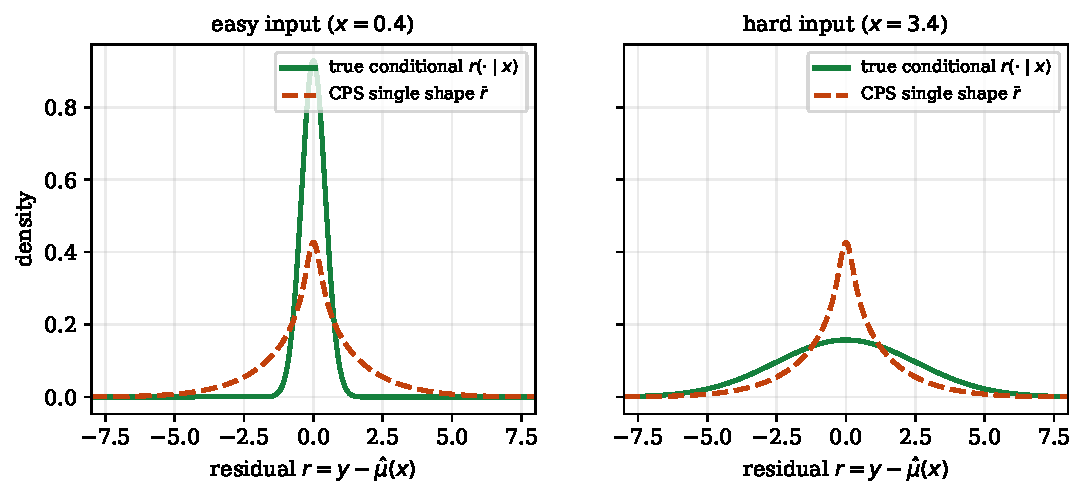
\includegraphics[width=0.92\textwidth]{fig_sharpness_gap.pdf}
\caption{Simulated illustration of Theorem~\ref{prop:residual}. A single input-blind
residual law serves every input, while the conditional residual law is narrow where the input is
easy and wide where it is hard. The log-score regret of the pooled system is $\I(R;X)$.}
\label{fig:gap}
\end{figure}

\subsection{Signed conformal predictive systems}\label{sec:cps}

A signed-residual conformal predictive system based on an independent calibration sample
estimates the full marginal residual CDF, with the usual finite-sample randomization details
\citep{vovk2019nonparametric}. Its $1-\alpha$ quantile, rank-adjusted to $\lceil(n+1)(1-\alpha)\rceil$, is the
corresponding one-sided split-conformal bound. Central intervals can be formed from two
signed-residual quantiles \citep{angelopoulos2025theoretical}. The usual symmetric two-sided
split-conformal interval instead pools absolute residuals, and it is treated in
Section~\ref{sec:abs}.

Under continuity and standard convergence conditions, the empirical
residual CDF converges to the marginal residual CDF $G$. Hence its large-calibration predictive
law converges to
\[
\Pi_x(y)=G\big(y-\hat\mu(x)\big).
\]
\begin{corollary}[Residual CPS information floor]\label{cor:cpsfloor}
Under the convergence conditions above, the population limit of the signed-residual CPS is the
marginal residual law $P_R$, the restricted optimum of Theorem~\ref{prop:residual}. If $P_R$
admits the required density, that limiting law has log-score regret $\I(R;X)$ relative to the
conditional residual oracle.
\end{corollary}

In misspecification language: conformal calibration consistently estimates the pseudo-true
member of a misspecified single-shape model, and consistency for the pseudo-truth does not
remove the model's specification error. This identifies the limiting law. It does not assert that the finite-sample CPS log risk
converges. That would require a smoothed predictive density and conditions such as KL
consistency, since empirical-CDF convergence alone does not control log score and the finite
empirical law is discrete.

\subsection{Absolute-residual intervals and symmetrization}\label{sec:abs}

In the population, or large-calibration, limit: if the nested family of ordinary
absolute-residual split-conformal intervals is interpreted as a predictive distribution by
sweeping the nominal level, the corresponding residual law is the symmetrization
\[
h_{\mathrm{sym}}(r)=\tfrac12\big\{\bar r(r)+\bar r(-r)\big\}.
\]
Its log-score regret is
\[
\I(R;X)+\KL(P_R\,\|\,H_{\mathrm{sym}}).
\]

The second term vanishes when the marginal residual law is symmetric. The symmetrization map can be interpreted as mixing $P_R$ with its reflection. The KL
penalty is bounded above by $\log 2$ whenever the relevant absolute-continuity conditions
hold.

\subsection{Coverage alone does not identify density quality}\label{sec:coverage}

A set-coverage guarantee does not by itself constrain the quality of a separately attached
density. Let $Y\sim N(0,1)$ and use the fixed score $s(y)=|y|$ to produce a split-conformal
interval. Attach instead the density $N(0,\sigma^2)$. The conformal interval and its coverage
are unchanged as $\sigma$ varies, while expected negative log score diverges to $+\infty$ as
$\sigma\downarrow0$ or $\sigma\uparrow\infty$. The observation is deliberately logical rather
than algorithmic: it shows that a set certificate cannot serve as evidence for the quality of a
density not used to construct the certificate \citep{recht2024cover}. It does not claim that
conformal predictive distributions themselves can be varied arbitrarily while holding their
construction fixed.

\subsection{Conditional ranks}\label{sec:ranks}

Assume the marginal residual CDF $G$ is continuous and strictly increasing on the support, and
let $U=G(R)$. Then $U$ is marginally uniform and the transformation is information preserving, so
\[
\I(R;X)=\I(U;X)=\E_X\KL\big(P_{U|X}\,\|\,\mathrm{Unif}[0,1]\big).
\]
With atoms one should use a randomized PIT. Without invertibility, data processing gives only
$\I(U;X)\le\I(R;X)$. Quantitative conditional-uniformity diagnostics can therefore provide variational or
classifier-based lower bounds on the representation floor. A hypothesis test alone does not
automatically estimate such a bound.

\subsection{Pooling in transformed coordinates}\label{sec:transformpool}

The empirical constructions of Section~\ref{sec:transformconform} pool residuals after a
state-dependent change of coordinates. The gap of any such scheme has a closed form.

\begin{theorem}[Transform pooling]\label{thm:transformpool}
For $P_X$-almost every $x$, assume:
\begin{enumerate}
\item $\phi_x:\mathbb R\to\mathcal Z$ is a strictly increasing $C^1$ diffeomorphism onto
a common open interval $\mathcal Z\subseteq\mathbb R$;
\item $(x,r)\mapsto\phi_x(r)$ and $(x,r)\mapsto\partial_r\phi_x(r)$ are jointly
measurable.
\end{enumerate}
Let $Z=\phi_X(R)$, and let $h$ be a density on $\mathcal Z$ with law $H$. A \emph{single
transformed-shape model} fixes one such $h$ and reports
\[
q_h(r\given x)=h\big(\phi_x(r)\big)\,\Big|\tfrac{\partial\phi_x(r)}{\partial r}\Big| .
\]
Then
\begin{equation}\label{eq:transformpool}
\E\log\frac{p(R\given X)}{q_h(R\given X)}=\I(Z;X)+\KL(P_Z\,\|\,H).
\end{equation}
The pseudo-true choice is $H=P_Z$, and the information gap of pooling in the coordinates
$\phi$ is $\I(Z;X)$.
\end{theorem}

\begin{proof}
Under the stated assumptions the change-of-variables formula gives, for each $x$,
\[
p(r\given x)=p_Z\big(\phi_x(r)\given x\big)\,\Big|\tfrac{\partial\phi_x(r)}{\partial r}\Big|,
\]
where $p_Z(\cdot\given x)$ is the conditional density of $Z=\phi_X(R)$ given $X=x$.
Dividing by the definition of $q_h$, the Jacobians cancel:
\[
\frac{p(R\given X)}{q_h(R\given X)}
=\frac{p_Z(Z\given X)\,|\partial_r\phi_X(R)|}{h(Z)\,|\partial_r\phi_X(R)|}
=\frac{p_Z(Z\given X)}{h(Z)}.
\]
Now insert the marginal density $p_Z$ of $Z$:
\[
\E\log\frac{p_Z(Z\given X)}{h(Z)}
=\E\log\frac{p_Z(Z\given X)}{p_Z(Z)}+\E\log\frac{p_Z(Z)}{h(Z)}
=\I(Z;X)+\KL(P_Z\,\|\,H),
\]
which is Theorem~\ref{prop:residual} applied to $Z$.
\end{proof}

\begin{remark}[Learned transformations]
If $\phi$ is learned from external training data $D$, independent of the test pair, apply
the theorem conditionally on $D$: the identity reads, as in Section~\ref{sec:learned},
$\E[\,\cdot\given D]=\I(Z;X\given D)+\KL(P_{Z|D}\,\|\,H_{D})$ with
$Z=\phi_{X,D}(R)$. For an online transformation whose state is generated from the current
preforecast filtration, include that state in $X$ or in $T$. Do not condition on the
entire
current history, which would fix the transformation and condition away the randomness being
priced.
\end{remark}

The theorem prices each pooling scheme by its coordinates: raw residual pooling has gap
$\I(R;X)$. Scale-normalized pooling has gap $\I(R/\hat\sigma(X);X)$. Pooling of
serially whitened residuals (the innovations $Z_{\mathrm{white}}$ left after an
autoregressive fit) has gap $\I(Z_{\mathrm{white}};X)$. Recalibration through a fitted
conditional CDF $\widehat F_x$ has gap $\I(U;X)$ with $U=\widehat F_X(Y)$, exactly when each
$\widehat F_x$ is strictly increasing and smooth onto a common range. Discrete or
noninvertible fitted CDFs would need a separate randomized-transform formulation, since a
randomized PIT is a stochastic kernel rather than a diffeomorphism. Absent such a
formulation, data processing gives only the corresponding information bound. It also exposes a
distinction that the next section's catalogue can blur: an architecture that estimates the full
conditional law $P_{R|\hat\sigma}$ has floor $\I(R;X\given\hat\sigma)$, whereas normalized
pooling imposes the stronger restriction that $R/\hat\sigma(X)$ has one common shape, and its
gap $\I(R/\hat\sigma(X);X)$ is in general different. They are not the same architecture.

\section{Representation-conditioned conformal methods}\label{sec:catalogue}

Let $T=T(X)$ be a representation used to stratify or normalize residuals. If an idealized method
estimates the full conditional residual law $P_{R|T}$, then its oracle floor is
$\I(R;X\given T)$. Examples include a finite partition, a scale state, or a learned embedding.
These examples are generally only partially ordered.

\begin{center}
\begin{tabular}{lll}
\toprule
Architecture & Residual representation & Oracle log-score floor\\
\midrule
Global residual pooling & constant & $\I(R;X)$\\
Group-wise (Mondrian) pooling & $B(X)$ & $\I(R;X\given B)$\\
Scale-conditioned residual model & $\hat\sigma(X)$ & $\I(R;X\given\hat\sigma)$\\
Learned residual state & $T_\theta(X)$ & $\I(R;X\given T_\theta)$\\
Full conditional residual model & sufficient $T$; in particular $X$ & $0$\\
\bottomrule
\end{tabular}
\end{center}

The table's floors price architectures that estimate the full conditional residual law given
the stated representation. Pooled-shape schemes are priced instead by
Theorem~\ref{thm:transformpool}. Conformalized quantile regression and methods based on
non-residual conformity scores fit most
cleanly into the general $(Z,T)$ theorem rather than automatically into the signed-residual
notation \citep{romano2019conformalized,chernozhukov2021distributional}. Their retained object
may be a vector of fitted quantiles and their calibrated target may be a scalar nonconformity
score. Any claim of an $\I(R;X\given T)$ floor should specify the residual or score variable
being predicted.

Conformalization at a fixed representation can alter $Q_{R|T}$ and hence the estimation term. It
may improve or worsen a proper score. It cannot change the lower bound $\I(R;X\given T)$ unless
the conformity construction itself changes $T$.

\section{Bayesian comparison of forecasting architectures}\label{sec:comparison}

Architecture comparisons depend on how plausible data-generating laws are weighted. Let
Nature draw a data-generating law $P\sim\Pi$, and let $\Dn$ be observed training data. Under
posterior predictive logarithmic loss, define the Bayes-optimal predictive law conditional on a
representation $T$ by $P_\Pi(Y\in\cdot\given T,\Dn)$. For a $T$-measurable forecast
$\widehat Q$, write
$\Loss_\Pi(\widehat Q\given\Dn)=-\E_\Pi\big[\log\widehat Q(Y\given T,\Dn)\given\Dn\big]$
for its posterior-predictive log risk and $\Loss^\star_\Pi(T\given\Dn)$ for the risk of the
Bayes-optimal choice. Information quantities subscripted by $\Pi$ are computed under the
joint
law induced by $\Pi$ given $\Dn$.

\begin{theorem}[Bayesian architecture comparison]\label{thm:bayes}
Let $T_A=g(T_B)$, so $T_B$ refines $T_A$. Conditional on $\Dn$, the difference between the
oracle posterior-predictive log risks is
\begin{equation}\label{eq:bayesoracle}
\Loss^\star_\Pi(T_A\given\Dn)-\Loss^\star_\Pi(T_B\given\Dn)
=\I_\Pi(Y;T_B\given T_A,\Dn).
\end{equation}
For fitted forecasts $\widehat Q_A$ and $\widehat Q_B$,
\begin{equation}\label{eq:bayesfitted}
\Loss_\Pi(\widehat Q_A\given\Dn)-\Loss_\Pi(\widehat Q_B\given\Dn)
=\I_\Pi(Y;T_B\given T_A,\Dn)+\epsilon_A(\Dn)-\epsilon_B(\Dn),
\end{equation}
where
$\epsilon_j(\Dn)=\E_\Pi\KL\big(P_\Pi(Y\given T_j,\Dn)\,\|\,\widehat Q_j(Y\given T_j,\Dn)\big)$.
Hence the richer architecture wins exactly when its added predictive information exceeds the
change in its within-representation excess risk.
\end{theorem}

\begin{proof}
Work under the joint law induced by $\Pi$, conditionally on $\Dn$. The Bayes-optimal
$T_j$-measurable predictive law is the posterior predictive $P_\Pi(Y\in\cdot\given
T_j,\Dn)$, and its log risk is the conditional entropy:
\[
\Loss^\star_\Pi(T_j\given\Dn)
=-\E_\Pi\big[\log p_\Pi(Y\given T_j,\Dn)\,\big|\,\Dn\big]
=H_\Pi(Y\given T_j,\Dn).
\]
Subtracting the two oracle risks and using $T_A=g(T_B)$, so that conditioning on $T_B$ is the
same as conditioning on $(T_A,T_B)$,
\[
\Loss^\star_\Pi(T_A\given\Dn)-\Loss^\star_\Pi(T_B\given\Dn)
=H_\Pi(Y\given T_A,\Dn)-H_\Pi(Y\given T_B,T_A,\Dn)
=\I_\Pi(Y;T_B\given T_A,\Dn),
\]
which is \eqref{eq:bayesoracle}. For fitted forecasts, Lemma~\ref{lem:voi} applied at each
$T_j$ under this law gives
$\Loss_\Pi(\widehat Q_j\given\Dn)=H_\Pi(Y\given T_j,\Dn)+\epsilon_j(\Dn)$.
Subtracting the two fitted risks and substituting \eqref{eq:bayesoracle} gives
\eqref{eq:bayesfitted}.
\end{proof}

Equation \eqref{eq:bayesfitted} gives the finite-sample architecture comparison at a fixed
prior and sample size. A coarse architecture has a
larger information floor but may be cheap to estimate. A richer architecture lowers the floor
but may have higher finite-sample error. No universal ordering exists without specifying the prior, sample size, and score.
Proposition~\ref{cor:bridge} is the rung-by-rung specialization of \eqref{eq:bayesfitted},
with the benchmark distribution in the role of $\Pi$. The ladder of Section~\ref{sec:ladder}
is an empirical realization of the full comparison: representation gain net of the change in
within-representation excess risk. Figure~\ref{fig:ladder} is that comparison at one point
of the map $\Pi\mapsto\{\Delta_j\}$.

\subsection{A two-regime prior favoring a tree-conditional learner}\label{sec:tworegime}

Let
\[
X\sim\mathrm{Bernoulli}(1/2),\qquad Y\given X{=}0\sim N(0,1),\qquad Y\given X{=}1\sim N(0,a^2),
\]
with $a\neq1$. The conditional mean is zero in both regimes. Thus a global residual predictor
and a conditional learner can share the same perfect point prediction.

The optimal pooled residual law is
\[
M_a=\tfrac12 N(0,1)+\tfrac12 N(0,a^2).
\]
A depth-one conditional tree can represent the two regime-specific laws. Its oracle log-score
advantage is
\begin{align}
\Delta(a)&=\tfrac12\KL\big(N(0,1)\,\|\,M_a\big)+\tfrac12\KL\big(N(0,a^2)\,\|\,M_a\big)
\label{eq:jsd}\\
&=\I(Y;X)>0.\nonumber
\end{align}
It equals the Jensen--Shannon divergence between the two conditional laws and is bounded above
by $\log2$. As the regimes become nearly distinguishable from the observation, $\Delta(a)$
approaches one bit per observation.

Now let the two variances be unknown. For every fixed true $a\neq1$, if the conditional
learner's excess KL risk vanishes and the pooled learner converges to $M_a$, then
\[
\lim_{n\to\infty}\big\{\Loss_a(\widehat Q_A)-\Loss_a(\widehat Q_B)\big\}=\Delta(a)>0 .
\]
Under a regular prior on the variances the same holds in prior-average risk with limit
$\E_\Pi[\Delta(A)]$, given posterior consistency and enough integrability to exchange the
limit with the prior average. At finite $n$, the conditional learner wins once the relevant
$\Delta$ exceeds its extra within-representation excess risk.
This is a concrete theoretical reason that boosted distributional trees, quantile boosting,
NGBoost, or separate boosted mean-and-scale models can outperform global residual conformal
prediction under priors assigning substantial mass to piecewise-learnable conditional
heteroscedasticity \citep{friedman2001greedy,chen2016xgboost,duan2020ngboost}.

The comparison is between prediction devices under the same score. Conformalization can be
attached to the richer learner, but a global residual-pooling output remains a coarser
predictive architecture than a model whose conditional scale or shape varies with $X$.

\section{Time series and retained state}\label{sec:timeseries}

Let $(Y_t)$ be a process and let $\F_{t-1}$ be the information available before predicting
$Y_t$. Let $\hat\mu_t$ be $\F_{t-1}$-measurable and define $R_t=Y_t-\hat\mu_t$. An architecture
retains a state
\[
T_t=T(\F_{t-1}).
\]
The one-step log-score decomposition is
\begin{equation}\label{eq:tsdecomp}
\E\log\frac{p(R_t\given\F_{t-1})}{q(R_t\given T_t)}
=\I(R_t;\F_{t-1}\given T_t)+\E\KL\big(P_{R_t|T_t}\,\|\,Q_{R_t|T_t}\big).
\end{equation}
Thus $\I(R_t;\F_{t-1}\given T_t)$ is the predictive information in the past omitted by the
retained state.

If the process is stationary, the relevant differential entropies are finite, and $\F_{t-1}$ is
generated by the residual past, then the pooled-state floor is
\[
\I(R_0;R_{-1},R_{-2},\dots)=h(R_0)-h(R_0\given R_{-1},R_{-2},\dots).
\]
This is the gap between marginal residual entropy and the one-step conditional entropy rate. If
the filtration includes exogenous variables or other information, the floor can be larger than
the residual-past entropy-rate gap.

If the state map or its hyperparameters are learned from external training data $D$, apply
\eqref{eq:tsdecomp} conditionally on $D$, or on a fixed initialization, with
$T_t=T_D(\F_{t-1})$. The current preforecast filtration $\F_{t-1}$ remains random.
Conditioning on the full current history would fix $T_t$ and condition away exactly the
randomness being measured. In nonstationary settings the one-step
conditional decomposition remains meaningful, but the stationary entropy-rate identity need not
hold. A linear-Gaussian state-space model is the extreme of representation efficiency: the
filtering posterior is a finite-dimensional sufficient statistic of the past
\citep{kalman1960new}, so its floor is zero, given known parameters and correctly specified
dynamics. Under parameter uncertainty the sufficient state must also carry the posterior over
parameters.

\subsection{Volatility as an information state}\label{sec:volatility}

Let returns satisfy
\[
Y_t=\sigma_t\varepsilon_t,\qquad \varepsilon_t\overset{\mathrm{iid}}{\sim}N(0,1),
\]
where $\sigma_t>0$ is $\F_{t-1}$-measurable, $\varepsilon_t$ is independent of
$\F_{t-1}$, $\E|\log\sigma_t|<\infty$, and the marginal entropy below is finite. The
conditional law is $N(0,\sigma_t^2)$. Global
pooling sees the scale mixture $\bar P$. Its representation floor is
\[
\I(Y_t;\F_{t-1})=h(\bar P)-\tfrac12\log(2\pi e)-\E\log\sigma_t .
\]
A volatility state $\hat\sigma_t$ has floor $\I(Y_t;\F_{t-1}\given\hat\sigma_t)$. This floor is
zero precisely when the retained state determines the true conditional scale, i.e.\ when
$\sigma_t$ is measurable with respect to $\hat\sigma_t$. Equality $\hat\sigma_t=\sigma_t$ is
sufficient but not necessary.

The practical point is concrete here. Heavy tails in the pooled return distribution
can arise because a single law mixes easy and hard volatility states. A volatility model reduces
the representation floor by distinguishing those states. A conformal normalization may then
certify quantiles or sets at the retained-state resolution, but the predictive gain comes from
the volatility state and the fit, not from the coverage statement by itself.

\section{Certification and conditional impossibility}\label{sec:certification}

Coverage is a property of sets or events, not a proper score for a complete predictive density.
A conformal certificate can be extremely valuable when the decision problem explicitly rewards
control of a miss rate, false-positive rate, or risk functional
\citep{vovk2005algorithmic,angelopoulos2021uncertainty,bates2021distribution,angelopoulos2024conformalrisk}.
It should nevertheless be accounted for separately from representation and estimation.

For a conformalized predictor with representation $T$, a useful ledger is:
\[
\text{predictive regret}=\text{representation regret}+\text{estimation/post-processing regret},
\]
plus a separate statement describing the coverage or risk certificate. The certificate may
constrain or change the second term. It does not alter the first unless the method changes
$T$.

Conditional-coverage no-go theorems state that exact, nontrivial, distribution-free conditional
coverage cannot be guaranteed at arbitrary resolution over rich distribution classes
\citep{lei2014distribution,barber2021limits}. The information theorem states that coarse
representations leave predictive information unused. Together they suggest a design tension, but
not a one-dimensional identity. Fine certification difficulty depends not only on
$\I(Y;X\given T)$ but also on the complexity and mass structure of $T$, the class of protected
subgroups, and the assumptions on the data-generating process.

A more complete methodological objective would minimize something of the form
\[
\underbrace{\I(Y;X\given T)}_{\text{oracle representation cost}}
+\underbrace{\mathrm{WithinRepErr}(T,\mathcal Q,n)}_{\text{model-form and fitting cost}}
+\underbrace{\lambda\,\mathrm{CertCost}(T,n,\alpha)}_{\text{certification cost}},
\]
where $\I(Y;X\given T)$ becomes $\mathcal I_S(Y;X\given T)$ when the scoring rule is not
log score, and the last term is the statistical cost of providing the certificate at level
$\alpha$. Any decision value the certificate delivers belongs on the benefit side of the
underlying decision problem, not in this risk sum. The weight $\lambda$ is
decision-specific. The optimal $T$ depends on the prior on Nature, the sample size, the
evaluation loss, and the utility assigned to certification.

The objective $\inf_T\{\I(Y;X\given T)+\lambda\,C(T)\}$ is a family of model-selection
criteria indexed by the complexity penalty. Taking $C(T)=\I(X;T)$ recovers the information
bottleneck \citep{tishby1999information}. Dimension, partition cardinality, VC-type
complexity, or expected excess risk give criteria in the spirit of penalized likelihood
\citep{akaike1974new}. Finite-sample estimation and certification cost need not coincide with
$\I(X;T)$, which is why we keep the penalty abstract.

\section{Asymptotic suboptimality of pooled residual architectures}\label{sec:deadend}

Is coverage-driven residual prediction a dead end? As a universal statement, no. As a complete
probabilistic forecasting architecture, global residual pooling can be asymptotically dominated
under broad structured priors.

Suppose a prior $\Pi$ concentrates on problems with learnable conditional residual structure
and satisfies
\[
\E_\Pi\,\I(R;X)\ge c>0,\qquad \E_\Pi\,\I(R;X\given T_B)\le d,
\]
where $T_B$ is the richer architecture's retained representation, and let both methods share
one fixed point predictor, so that $R$ and hence $\I(R;X)$ do not depend on the method or
the sample size. Define the prior-average risk advantage
$A_n:=\Loss_{\Pi,n}(\widehat Q_{\mathrm{pooled}})-\Loss_{\Pi,n}(\widehat
Q_{\mathrm{rich}})$. Suppose both learners converge in prior-average log risk to their
architecture-specific pseudo-truths. The pooled learner's limiting risk exceeds the
conditional oracle's by $\E_\Pi\I(R;X)$ and the richer learner's by
$\E_\Pi\I(R;X\given T_B)$, so the advantage converges:
\[
A_n\;\longrightarrow\;\E_\Pi\big[\I(R;X)-\I(R;X\given T_B)\big]\;\ge\;c-d,
\qquad\text{hence}\qquad \liminf_n A_n\ge c-d.
\]
The richer architecture recovers the pooled gap up to its own remaining floor. The conclusion
is a positive domination statement only when $c>d$. If the richer learner
consistently estimates the full conditional residual law, so that $d=0$, this holds
automatically, and for every $\eta>0$ the advantage eventually exceeds $c-\eta$. Under such
a prior,
global residual pooling is not Bayes-optimal as a prediction device, even though its conformal
intervals retain exact marginal coverage under exchangeability.

This is the relevant sense in which coverage-driven residual prediction may be a dead end.
The coverage theorem is true. The architecture nevertheless pays a persistent
predictive-information cost that realistic conditional learners can eventually overcome.
Conversely, at small samples or under a prior close to $R\perp X$, the pooled architecture can
lie near the optimum because its information floor is small and its estimation burden is
minimal.

Conformal methods remain compelling when the certificate itself has decision value: selective
prediction with abstention, risk control, regulatory reporting, anomaly testing, or safety
systems with fallback actions
\citep{angelopoulos2021uncertainty,bates2021distribution,angelopoulos2024conformalrisk}. In
those applications the correct comparison is not a proper score alone but the full utility of
the certified decision rule. A coverage guarantee does not remove the relevance of predictive scoring, and predictive
underperformance does not make a coverage certificate worthless.
The decomposition identifies which value is being purchased and what it costs.

\section{Conclusion}\label{sec:conclusion}

The exact result is a decomposition. A forecasting architecture exposes a representation $T$
to its predictive law, and under log loss the cost of the restriction is the information gap
$\I(Z;X\given T)$ plus a within-representation excess. For residual systems the gap of pooling
after a state-dependent invertible transformation $\phi_X$ is $\I(\phi_X(R);X)$, so the
irreducible cost of pooled residual prediction is determined by the coordinates in which
pooling occurs. Conformal calibration can improve the excess and supply a certificate. It cannot reduce
the gap without changing the retained representation.

The empirical result is an attribution. On this benchmark, conditional scale is the principal residual state omitted by raw
pooling. The finding survives a matched-predictor comparison, an i.i.d.\ simulation of the
certificate itself, and replication on an out-of-development holdout. Scale is also the
largest component in a same-game Shapley analysis of the surrogate coalition system on 234
series. With the point predictor held fixed,
scale-normalized empirical pooling was the best construction we tested under the
quantile-approximated CRPS.

The design principle follows. Choose the representation, the residual-law estimator, and the
certificate jointly, under the scoring rule and the prior that describe the problem. The
useful question is therefore not whether calibration or machine learning is universally
superior. It is which representation, estimator, and certificate jointly minimize the
decision-maker's risk under the problems Nature is believed to generate.

\section*{Code and data availability}
\ifanon
Code and data references are withheld for double-blind review and will be restored on
acceptance. The experiments are Python scripts against a public online-forecasting library;
script names match the labels used in the text.
\else
\begin{sloppypar}
 The decomposition arithmetic of Theorem~\ref{prop:residual} is checked numerically by
\texttt{check\_gap.py} on a heteroscedastic Gaussian and a skewed residual law; the check
exercises the algebra on a worked example rather than simulating the conformal procedures. Figures are generated by \texttt{figures.py} and \texttt{fig\_ladder.py}, and the
simulation by \texttt{check\_conformal\_sim.py}. All live at
\url{https://github.com/microprediction/conformalprediction}. The experiments are Python scripts in the \texttt{benchmarks} directory of the
\texttt{skaters} repository \citep{cotton_skaters}. They are named \texttt{ladder\_ablation}, \texttt{shapley\_ladder},
\texttt{ladder\_holdout}, \texttt{leaf\_bakeoff}, \texttt{conformal\_infogap}, and
\texttt{conformal\_decomposition}. The corpus enumeration, continuity filter, and scoring conventions
follow that repository's published benchmarks.
\end{sloppypar}
\fi

\appendix

\section{Terminal-leaf bake-off}\label{app:bakeoff}

In the grid of Section~\ref{sec:transformconform}, scale-normalized empirical pooling beat
the complete forecaster's fitted density under the quantile-approximated CRPS, while under
the log score the ladder showed the complete forecaster well ahead. This appendix asks the finer,
leaf-level question: holding the whitened residual stream fixed, which terminal law should
one attach?

Empirical pooling has one limitation that no choice of coordinates removes: it says nothing
about tails. The empirical distribution is a statement about where one has data, and it does
not extrapolate beyond its observed extremes. High quantiles simply equal the sample maximum. An
unsmoothed empirical measure is not directly usable as a continuous log-density forecast,
since it assigns zero density off its support. Tail mass is unobserved by definition, so
quoting it requires an assumption, whatever machinery carries it. A conformalized parametric
or semiparametric model can carry tail mass, with the shape supplied by assumption rather
than by distribution-free information.

The conformal literature's implicit answer is restraint: at calibration levels finer than
$1/(n{+}1)$, distribution-free validity requires an infinite or trivial endpoint, or suitable
randomization, so nontrivial finite bounds stop at the calibration resolution. That serves the coverage guarantee and forfeits density evaluation.

The semi-parametric synthesis is to pool the body empirically and model the tail: an
empirical law where data is dense, spliced to a peaks-over-threshold tail where it is sparse.
Extreme value theory supplies one principled asymptotic family of assumptions for that
region. Under CRPS and integrated quantile scores the tail choice matters little, since those
scores penalize location errors roughly linearly and have little far-tail density
sensitivity. Under the log score it is decisive. This is one more instance of the scoring rule determining the design. We document here a bake-off of terminal leaves, on the same whitened residual stream, that
sharpens that finding.
The protocol matches the grid: the same 701 series and fixed mean, the same EWMA scale and
AR(1) whitening, and CRPS on the common quantile grid. For the log score every leaf is a
genuine density. Empirical variants are smoothed by a binned Gaussian kernel with Silverman
bandwidth. Generalized Pareto (GPD) tails are fitted by moments to exceedances beyond the
$95\%$ thresholds. The conformal tail completion leaves all observed data empirical and
shapes only the reserved $1/(n{+}1)$ mass with the GPD. Scripts and per-series results accompany the paper.

\begin{center}
\small
\begin{tabular}{lccc}
\toprule
Terminal leaf & CRPS rel.\ Gaussian & log score $-$ Gaussian & beats Gaussian\\
 & mean / median & mean / median (nats/obs) & (log score)\\
\midrule
Gaussian, EWMA variance & $1.000$ / $1.000$ & $0$ / $0$ & \\
fitted scale mixture & $1.161$ / $1.000$ & $+0.10$ / $+0.011$ & $79\%$\\
empirical & $0.936$ / $0.985$ & $+0.19$ / $+0.023$ & $84\%$\\
windowed empirical (300) & $0.936$ / $0.986$ & $+0.18$ / $+0.020$ & $79\%$\\
empirical $+$ GPD tails & $0.938$ / $0.986$ & $+0.21$ / $+0.034$ & $83\%$\\
conformal tail completion & as empirical & $+0.21$ / $+0.033$ & $90\%$\\
score-weighted leaf ensemble & $0.942$ / $0.987$ & $+0.22$ / $+0.043$ & $98\%$\\
\bottomrule
\end{tabular}
\end{center}

In the log-score columns positive numbers are improvements over the Gaussian leaf, in nats
per observation. Every leaf's log score is evaluated as a mixture with a common reference
Gaussian (weight $0.01$), so all columns are genuine log scores under one convention and no
leaf benefits from a private clamp. Means exceed medians because a minority of heavy-tailed
series dominate them. All bandwidths, thresholds, mixture weights, and GPD
fits are computed from past observations only, so every evaluation is strictly out of sample.

Under the quantile-approximated CRPS every empirical variant beats every fitted law. The
differences among empirical variants are a few tenths of a percent, and banded smoothing and
an online quantile tracker are indistinguishable from the plain empirical. Under a score with
little far-tail sensitivity the estimator class is what matters, and refinements are
cosmetic.

Under the log score the empirical leaves win as well, and the tails decide the margins. The
fitted mixture trails every empirical variant, the empirical body with GPD tails leads on
mean gain, and the conformal tail completion has the best win rate among single leaves
($90\%$) and is strongest on short series (median gain $+0.039$ nats per observation on
series shorter than $1200$, improving $86\%$ of them, against $+0.015$ on series longer than
$2500$). The best overall leaf is a decayed-score-weighted ensemble of the leaves themselves,
which beats the Gaussian on $98\%$ of series. A windowed empirical adds nothing over the
expanding one at any length: forgetting belongs in the scale state, not the leaf. Which finite-sample
validity properties survive when reserved mass is shaped by a fitted tail model is not
established here, and the tail-completion construction should be read as a predictive
proposal, not a certified one.

The bake-off compares estimator classes on a fixed whitened stream, and it invites a
package-level conclusion that turns out to be wrong. We implemented the empirical leaf and
the score-weighted leaf ensemble as terminal options inside the complete forecaster and
reran the comparison in situ, with every other component at its production setting
(\texttt{leaf\_insitu.py}). The swap improved nothing. On the same 701 series the
empirical leaf lost to the reference configuration under both scores (relative CRPS $1.03$,
winning $14\%$ of series; log score $-0.26$ nats per observation, winning $6\%$), and the
ensemble leaf was closer but still behind. The reconciliation is the three-price ledger of
Section~\ref{sec:ladder}: the reference system already realizes the empirical advantage
through its CRPS-fitted terminal leaf and its tail splice, so the model-form gain the
bake-off measures has already been spent. The idea of residual pooling did not, in this case,
improve the shipped model even after all the conditional modeling was done.

\section{Deferred proofs}\label{app:proofs}

\paragraph{Proof of Proposition~\ref{cor:bridge}.}
Apply Lemma~\ref{lem:voi} conditionally on $\Dn$ at rung $j$: the log risk of
$\widehat Q_j$ splits as
\[
\widehat\Loss(\widehat Q_j)=H(Y\given T_j,\Dn)+\epsilon_j(\Dn),
\]
oracle entropy plus within-representation excess, and likewise at rung $j-1$. Subtracting,
\[
\Delta_j=\big[H(Y\given T_{j-1},\Dn)-H(Y\given T_j,\Dn)\big]
+\epsilon_{j-1}(\Dn)-\epsilon_j(\Dn).
\]
Because $T_{j-1}$ is a function of $T_j$, conditioning on $T_j$ is the same as conditioning
on $(T_j,T_{j-1})$, so
\[
H(Y\given T_{j-1},\Dn)-H(Y\given T_j,\Dn)
=H(Y\given T_{j-1},\Dn)-H(Y\given T_j,T_{j-1},\Dn)
=\I(Y;T_j\given T_{j-1},\Dn),
\]
which is Corollary~\ref{cor:nested} in entropy form.

\paragraph{Proof of Proposition~\ref{prop:cumulative}.}
Sum \eqref{eq:bridge} over $j=1,\dots,m$. The excess-risk terms telescope to
$\epsilon_0(\Dn)-\epsilon_m(\Dn)$. For the information terms, write each as an entropy
difference as in the previous proof and telescope again:
\[
\sum_{j=1}^m\I(Y;T_j\given T_{j-1},\Dn)
=\sum_{j=1}^m\big[H(Y\given T_{j-1},\Dn)-H(Y\given T_j,\Dn)\big]
=H(Y\given T_0,\Dn)-H(Y\given T_m,\Dn).
\]
By Corollary~\ref{cor:nested} applied to the pair $(T_0,T_m)$ with $T_0=g(T_m)$,
\[
H(Y\given T_0,\Dn)-H(Y\given T_m,\Dn)
=\I(Y;T_m\given T_0,\Dn)
=\I(Y;X\given T_0,\Dn)-\I(Y;X\given T_m,\Dn),
\]
which gives \eqref{eq:cumulative}. Adding and subtracting $\I(Y;X\given T_m,\Dn)$ in the
telescoped sum gives the remainder form \eqref{eq:remainder}.


\small
\bibliographystyle{plainnat}
\bibliography{references}

\end{document}
